\documentclass[12pt,a4paper]{report}

% ============================ 预加载的 LaTeX 包 ============================
\usepackage[a4paper,left=3.5cm,right=3cm,top=3cm,bottom=3cm]{geometry}
\usepackage[protrusion=true,expansion=true]{microtype}
\usepackage{setspace}
\usepackage{fancyhdr}
\usepackage{newtxtext,newtxmath}
\usepackage{amsmath, amssymb, amsthm}
\usepackage{graphicx}
\usepackage{listings}
\usepackage{xcolor}
\usepackage{multicol}
\usepackage[toc,page]{appendix}
\usepackage{tocbibind}
\usepackage{caption}
\usepackage{xcolor}
\usepackage{titlesec}
\usepackage{eso-pic}
\usepackage{tikz}
\usepackage{datetime}
\usepackage{tocloft}
\usepackage{titletoc}
\usepackage{cite}
\usepackage{lipsum}
\usepackage{etoolbox}
\usepackage{ragged2e}

% ================================= 设置公式 ================================
\AtBeginEnvironment{equation}{\setstretch{1}}
\AtEndEnvironment{equation}{}
\numberwithin{equation}{section}
\renewcommand{\theequation}{\arabic{section}.\arabic{equation}}

% ================================= 设置页脚 ================================
\pagestyle{fancy}
\fancyhf{}
\fancyfoot[R]{\fontsize{12pt}{14pt}\selectfont \thepage}
\renewcommand{\headrulewidth}{0pt}
\fancypagestyle{plain}{
    \fancyhf{}
    \fancyfoot[R]{\fontsize{12pt}{14pt}\selectfont \thepage}
    \renewcommand{\headrulewidth}{0pt}
}

% ================================= 设置目录 ================================
\def\contentsname{}
\newcommand{\customtoc}{
    \clearpage
    \begin{center}
        \underline{\textbf{\fontsize{18pt}{18pt}\selectfont Table of Contents}}
    \end{center}
    \vspace{-1.2\baselineskip}
}
% 自定义 "Pages" 列标题，使其右对齐
\makeatletter
\@ifpackageloaded{tocloft}{}{
  \usepackage{tocloft}
}
\makeatother
\makeatletter
\@ifpackageloaded{titletoc}{}{
  \usepackage{titletoc}
}
\makeatother
\makeatletter
\providecommand*\cftaftertoctitle{}
\makeatother
\@ifpackageloaded{tocloft}{}{
  \renewcommand{\cftaftertoctitle}{%
      \vspace{-1.5\baselineskip}
      \hfill\underline{Pages}
      \par\vskip-2\baselineskip
  }
}
% 目录格式调整
% 一级标题 (chapter) 设置
\makeatletter
\@ifpackageloaded{tocloft}{%
  \renewcommand{\cftchapfont}{\bfseries}
  \renewcommand\thechapter{Chapter\enspace\arabic{chapter}}
  \renewcommand\thesection{\arabic{chapter}.\arabic{section}}
  \renewcommand{\cftchapaftersnumb}{}
  \setlength{\cftchapnumwidth}{5.3em}
  % 二级标题（section）设置
  \renewcommand{\cftsecfont}{}
  \renewcommand{\cftsecpresnum}{}
  \renewcommand{\cftsecaftersnumb}{}
  \setlength{\cftsecindent}{0em}
  \setlength{\cftsecnumwidth}{2em}
  \renewcommand{\cftsecdotsep}{\cftnodots}
  % 间距设置
  \setlength{\cftbeforechapskip}{0.5em}
  \setlength{\cftbeforesecskip}{0.5em}
}{}
\makeatother

% ========================== 统一设置 \chapter ==========================
\titleformat{\chapter}[display]
  {\normalfont\Huge\bfseries}
  {\thechapter}
  {0em}
  {\raggedright}
\titleformat{name=\chapter,numberless}[display]
  {\normalfont\Huge\bfseries}
  {}
  {-2.5em}
  {\centering}
\titlespacing{\chapter}{0pt}{-2em}{0em}
\titlespacing{name=\chapter,numberless}{0pt}{0em}{\baselineskip}

% ========================== 统一设置 \section ==========================
\titleformat{\section}
  {\normalfont\fontsize{16pt}{16pt}\bfseries}
  {\thesection\enspace}
  {0pt}
  {\raggedright}
\titleformat{name=\section,numberless}[display]
  {\clearpage\normalfont\fontsize{16pt}{16pt}\bfseries}
  {}
  {-1em}
  {\centering}
\titlespacing{\section}{0pt}{0.5\baselineskip}{0.5\baselineskip}
\titlespacing{name=\section,numberless}{0pt}{0em}{1.5\baselineskip}

% ======================= 统一设置 \subsection ========================
\titleformat{\subsection}
  {\normalfont\fontsize{14pt}{14pt}\bfseries}
  {\thesubsection\enspace}
  {0pt}
  {\raggedright}
\titlespacing{\subsection}{0pt}{0.5\baselineskip}{0.5\baselineskip}

\global\sloppy

\begin{document}

\onehalfspacing

% ================================ 自定义颜色 ================================
\definecolor{DeepGreen}{rgb}{0.0, 0.690, 0.314}

% ================================ 自定义设置 ================================
% 左缩进为0
\setlength{\parindent}{0pt}
% 自定义日期格式
\newdateformat{mydate}{\THEDAY\ \monthname[\THEMONTH]\ \THEYEAR}
% 让图编号显示为 "Figure X.Y"
\makeatletter
\@ifpackageloaded{hyperref}{}{
  \usepackage{hyperref}
}
\makeatother
\makeatletter
\AtBeginDocument{%
  \@ifpackageloaded{hyperref}{%
    \renewcommand{\thefigure}{Figure \arabic{chapter}.\arabic{figure}}%
  }{%
    \renewcommand{\thefigure}{Figure \arabic{chapter}.\arabic{figure}}%
  }%
}
\makeatother
\makeatletter
\@ifpackageloaded{tocloft}{%
  \setlength{\cftfignumwidth}{4.5em}
}{}
\makeatother
\makeatletter
\@ifpackageloaded{hyperref}{}{%
  \setlength{\cftfignumwidth}{4.5em}
}{}
\makeatother
% 让表格编号显示为 "Table X.Y"
\makeatletter
\AtBeginDocument{%
  \@ifpackageloaded{hyperref}{%
    \renewcommand{\thetable}{Table \arabic{chapter}.\arabic{table}}%
  }{%
    \renewcommand{\thetable}{Table \arabic{chapter}.\arabic{table}}%
  }%
}
\makeatother
\makeatletter
\@ifpackageloaded{tocloft}{%
  \setlength{\cfttabnumwidth}{4.5em}
}{}
\makeatother
\makeatletter
\@ifpackageloaded{hyperref}{}{%
  \setlength{\cfttabnumwidth}{4.5em}
}{}
\makeatother

% ======================== 论文前置部分（Front Matter） =======================
\pagenumbering{gobble}
\begin{titlepage}
    \centering

    % 第一页
    \vspace*{1cm}

    
\includegraphics[width=0.8\textwidth]{assets/ntu-logo.png} % NTU Logo

    \vspace*{6cm}

    \textbf{\LARGE Enhancing Code Error Classification with} \\
    \textbf{\LARGE Proximal Policy Optimization} \\
    \vspace{1cm}
    \textbf{\LARGE Based on Qwen2.5-Coder Model}

    \vfill

    \textbf{[Your Name]} \\
    \textbf{SCHOOL OF ELECTRICAL AND ELECTRONIC ENGINEERING} \\
    \textbf{2026}

    \vspace*{1cm}

    % 第二页
    \newpage

    \vspace*{6cm}

    \textbf{\LARGE Enhancing Code Error Classification with} \\
    \textbf{\LARGE Proximal Policy Optimization} \\
    \vspace{1cm}
    \textbf{\LARGE Based on Qwen2.5-Coder Model}

    \vfill

    \textbf{[Your Name]}

    \vfill

    \textbf{SCHOOL OF ELECTRICAL AND ELECTRONIC ENGINEERING}

    \vspace*{\baselineskip}

    \textbf{A DISSERTATION SUBMITTED IN PARTIAL FULFILMENT OF THE REQUIREMENTS FOR THE DEGREE OF} \\
    \textbf{MASTER OF SCIENCE IN} \\
    \textbf{SIGNAL PROCESSING AND MACHINE LEARNING}

    \vfill

    \textbf{2026}

    \vspace*{1cm}
\end{titlepage}

\input{c-front-matter/originality}
\input{c-front-matter/supervisor-declaration}
\section*{Authorship Attribution Statement}

Please select one of the following; *delete as appropriate:

\vspace{0.5\baselineskip}

*(A) This thesis does not contain any materials from papers published in peer-reviewed journals or from papers accepted at conferences in which I am listed as an author.

\vspace{0.5\baselineskip}

*(B) This thesis contains material from [x number] paper(s) published in the following peer-reviewed journal(s) / from papers accepted at conferences in which I am listed as an author.

\vspace{0.5\baselineskip}

\textcolor{DeepGreen}{\underline{
Please amend the typical statements below to suit your circumstances if (B) is selected.
}}

\vspace{1cm}

\noindent
\begin{center}
    \begin{tabular}{>{\centering\arraybackslash}p{6cm} p{1cm} >{\centering\arraybackslash}p{6cm}}
        \mydate\today &  &
        \begin{tikzpicture}
            \node[opacity=0.9, anchor=center] at (0,0) {
\includegraphics[width=5cm]{assets/ntu-watermark.png}};
            \node[anchor=north] at (0,2) {
\includegraphics[width=4cm]{signature/personal-signature.png}};
        \end{tikzpicture} \\
        \dotfill &  & \dotfill \\[0.2cm]
        Date &  & \textcolor{red}{Your Name} \\
    \end{tabular}
\end{center}


\clearpage
\thispagestyle{empty}
\begin{center}
\vspace*{2cm}
\textbf{\Large Table of Contents}
\end{center}
\vspace{1cm}
\tableofcontents
\clearpage

\clearpage
\pagenumbering{roman}
\chapter*{Abstract}
\addcontentsline{toc}{chapter}{Abstract}
\chapter*{Abstract}
\addcontentsline{toc}{chapter}{Abstract}
\begingroup
\justifying
\setlength{\parindent}{0pt}
\setstretch{2}
\setlength{\parskip}{0.5\baselineskip}

Automatic code error classification is a critical task in software engineering and automated debugging systems. With the rapid advancement of large language models (LLMs), particularly code-specialized models such as Qwen2.5-Coder, there is growing interest in leveraging these models for multi-label code error type prediction. However, the vanilla fine-tuning approach often fails to capture the nuanced relationships between error patterns and their corresponding labels, leading to suboptimal classification performance.

In this thesis, we propose a novel approach that combines the Qwen2.5-Coder-1.5B-Instruct model with Proximal Policy Optimization (PPO), a reinforcement learning algorithm, to enhance multi-label code error classification. Specifically, we formulate the error classification task as a sequence generation problem, where the model generates error type labels given error code snippets. We employ two discriminator models---a fluency discriminator and an alignment discriminator---to provide reward signals. The fluency discriminator evaluates whether the generated label sequence is syntactically and semantically coherent, while the alignment discriminator assesses whether the predicted labels correctly match the underlying error patterns in the code.

Our experimental results on a dataset of Python code errors demonstrate that the proposed PPO-based approach achieves a micro F1 score improvement from 60.6\% to 62.5\% over the base model, validating the effectiveness of reinforcement learning fine-tuning for code error classification tasks.

\textbf{Keywords:} Code Error Classification, Multi-label Classification, Qwen2.5-Coder, Proximal Policy Optimization, Reinforcement Learning, Large Language Models

\endgroup

\chapter*{Acknowledgements}
\addcontentsline{toc}{chapter}{Acknowledgements}
\chapter*{Acknowledgements}
\addcontentsline{toc}{chapter}{Acknowledgements}
\begingroup
\justifying
\setlength{\parindent}{0pt}
\setstretch{2}
\setlength{\parskip}{0.5\baselineskip}

I would like to express my deepest gratitude to my supervisor for their invaluable guidance, patient encouragement, and constructive feedback throughout the course of this research. Their expertise and insights have been instrumental in shaping this dissertation.

I am also grateful to the members of our research group for their stimulating discussions and helpful suggestions. Special thanks go to all my colleagues who provided technical support and shared their knowledge during the development of this project.

Finally, I would like to thank my family and friends for their unwavering support and understanding during the entire duration of this work.

\endgroup

\listoffigures
\listoftables

% ========================= 论文正文部分（Main Content） ========================
\clearpage
\pagenumbering{arabic}
\chapter{Introduction}
\begingroup
\justifying
\setlength{\parindent}{0pt}
\setstretch{2}
\setlength{\parskip}{0.5\baselineskip}
\titlespacing{\chapter}{0pt}{0pt}{0pt}
\titlespacing{\section}{0pt}{0pt}{0pt}

\section{Motivation and Background}

Software debugging is one of the most time-consuming and costly activities in software development. Among the various challenges in automated debugging, accurately classifying code errors into their respective types stands as a fundamental yet critical step. Precise error classification enables developers to quickly understand the nature of bugs, prioritize fixing efforts, and even automate remediation processes. Traditional rule-based error classification systems often struggle with the diversity and complexity of real-world code errors, necessitating more sophisticated machine learning approaches.

In recent years, large language models (LLMs) have demonstrated remarkable capabilities across a wide range of natural language and code understanding tasks. Models such as GPT-4 \cite{openai2023gpt4}, CodeLlama \cite{roziere2023code}, and Qwen-Coder \cite{qwen2024coder} have shown strong performance in code generation, explanation, and analysis tasks. These models, pre-trained on massive corpora of code and text, possess rich representations of programming concepts and syntactic patterns. Fine-tuning these models for specific downstream tasks has become a standard paradigm in applied machine learning.

However, the naive fine-tuning approach, which typically employs supervised learning with cross-entropy loss, may not fully capture the nuanced relationships between code error patterns and their corresponding error types. In particular, for multi-label classification tasks where a code snippet may contain multiple error types simultaneously (e.g., both a logical error and an omission), the standard next-token prediction objective does not provide direct feedback on whether the generated label sequence is coherent, aligned with the input code, or consistent across different error categories.

To address these limitations, we propose leveraging reinforcement learning (RL) to fine-tune a code-specialized LLM for error classification. Specifically, we employ Proximal Policy Optimization (PPO) \cite{schulman2017proximal}, an RL algorithm widely used for training language models, to refine the model's error classification capabilities. The key insight is that by introducing reward signals from discriminator models that evaluate both the fluency of generated labels and their alignment with the input error code, we can guide the model toward producing more accurate and coherent predictions.

This thesis focuses on the task of multi-label code error type classification using Qwen2.5-Coder-1.5B-Instruct, a 1.5 billion parameter instruction-tuned model specialized for code tasks. We investigate how PPO-based fine-tuning, combined with fluency and alignment discriminators, can improve classification performance beyond supervised fine-tuning baselines.

\section{Problem Statement}

Given a code snippet containing one or more errors, the task is to predict a set of error type labels from a predefined taxonomy. The error type taxonomy in this work includes six categories:

\begin{itemize}
    \item \textbf{Logical Error}: The code executes without crashing but produces incorrect results due to flawed logic.
    \item \textbf{Memory Error}: The code contains memory-related issues such as out-of-bounds access or memory leaks.
    \item \textbf{Omission}: The code is missing necessary components (e.g., a return statement, a condition check).
    \item \textbf{Invalid Condition}: The code contains conditional statements that evaluate incorrectly under certain inputs.
    \item \textbf{Infinite Loop Error}: The code enters an infinite loop due to improper loop conditions or missing loop termination.
    \item \textbf{Unknown}: Error types that do not fall into the above categories.
\end{itemize}

This is fundamentally a multi-label classification problem, as a single code snippet may exhibit one or more of these error types simultaneously. The evaluation metric is multi-label classification performance, with micro F1 and macro F1 as the primary metrics.

Formally, let $x$ denote an input code snippet and $y \subseteq \mathcal{L}$ denote the set of true error labels, where $\mathcal{L} = \{\text{logical\_error}, \text{memory\_error}, \text{omission}, \text{invalid\_condition}, \text{infinite\_loop\_error}, \text{unknown}\}$. The goal is to learn a model $f: \mathcal{X} \rightarrow 2^{\mathcal{L}}$ that maps code snippets to sets of error labels.

\section{Objectives and Scope}

The primary objectives of this thesis are as follows:

\begin{enumerate}
    \item To develop a PPO-based reinforcement learning framework for fine-tuning the Qwen2.5-Coder model on the multi-label code error classification task.
    \item To design and train discriminator models that evaluate the fluency and alignment of generated error labels, serving as reward signals in the PPO framework.
    \item To conduct comprehensive experiments comparing the PPO fine-tuned model against supervised fine-tuning baselines, analyzing performance across different error categories.
    \item To investigate the impact of different training configurations, including discriminator architectures, reward scaling, and PPO hyperparameters, on classification performance.
\end{enumerate}

The scope of this thesis is limited to Python code error classification, as Python is one of the most widely used programming languages and features distinct error patterns compared to compiled languages. We focus on the Qwen2.5-Coder-1.5B-Instruct model due to its balance of performance and computational efficiency.

\section{Contributions}

The main contributions of this thesis are summarized as follows:

\begin{itemize}
    \item We propose a novel approach that combines Qwen2.5-Coder with PPO-based reinforcement learning for multi-label code error classification. To the best of our knowledge, this is the first work to apply PPO fine-tuning to the code error classification task using a code-specialized LLM.
    \item We introduce a dual-discriminator reward framework consisting of a fluency discriminator and an alignment discriminator. These discriminators provide complementary reward signals that guide the model toward generating fluent and accurate error label sequences.
    \item We conduct extensive experiments on a real-world Python code error dataset, demonstrating that the proposed PPO-based approach achieves a significant improvement in micro F1 score (from 60.6\% to 62.5\%) compared to the base model.
    \item We provide a detailed analysis of the experimental results, including per-error-type performance, the effect of discriminator training, and qualitative examples of generated labels.
\end{itemize}

\section{Thesis Organization}

The remainder of this thesis is organized as follows:

\begin{itemize}
    \item Chapter 2 provides a comprehensive review of related work, covering large language models for code, multi-label text classification, and reinforcement learning for language model training.
    \item Chapter 3 describes the proposed methodology in detail, including the base model, the PPO framework, the discriminator architectures, and the reward computation mechanism.
    \item Chapter 4 presents the experimental setup, datasets, evaluation metrics, and results.
    \item Chapter 5 discusses the findings, limitations, and potential directions for future work.
    \item Chapter 6 concludes the thesis.
\end{itemize}

\endgroup
\endinput

\chapter{Related Work}
\begingroup
\justifying
\setlength{\parindent}{0pt}
\setstretch{2}
\setlength{\parskip}{0.5\baselineskip}
\titlespacing{\chapter}{0pt}{0pt}{0pt}
\titlespacing{\section}{0pt}{0pt}{0pt}

\section{Automated Program Repair}

Automated Program Repair (APR) aims to automatically fix bugs in source code without human intervention. Traditional repair techniques rely on pre-defined fix templates or search-based algorithms~\cite{zhang2023surveylearningbasedautomatedprogram}. With the advancement of deep learning, learning-based APR has emerged as a dominant approach, modeling bug fixing as a sequence-to-sequence translation task where buggy code is translated into fixed code~\cite{zhang2023surveylearningbasedautomatedprogram}. The typical pipeline consists of three stages: fault localization to identify buggy code locations, patch generation to produce candidate fixes, and validation to verify correctness.

Recent work has incorporated syntactic constraints to ensure generated patches are syntactically valid. \textit{Recoder} proposes a syntax-guided edit decoder that generates edits rather than entire code, significantly improving efficiency and correctness~\cite{zhu2022syntaxguidededitdecoderneural}. By leveraging Abstract Syntax Trees (ASTs), this approach constrains the generation space to syntactically valid modifications. Template-based methods like GAMMA combine fix templates with masked language models, achieving strong performance by transforming templates into mask patterns for context-aware prediction~\cite{zhang2023gammarevisitingtemplatebasedautomated}. However, these approaches face a trade-off between controllability and flexibility: templates provide predictable fixes but limit the diversity of generated patches.

Multi-source approaches have also been explored to improve repair performance. Prior work incorporates AST structures, code comments, and other contextual information as inputs to pre-trained code models~\cite{paul2023enhancingautomatedprogramrepair}. These methods demonstrate that structural information enhances semantic understanding and leads to more accurate repairs.

While existing work primarily focuses on fixing bugs, there is limited research on generating them in a controllable manner. This thesis addresses this gap by proposing a framework that generates buggy code conditioned on error types, enabling fine-grained control over the generation process.

\section{Abstract Syntax Tree Based Code Understanding}

Abstract Syntax Trees (ASTs) provide a hierarchical representation of code structure that captures both syntactic and semantic information. Unlike raw token sequences, ASTs encode the grammatical relationships between code elements, making them particularly useful for tasks requiring structural understanding.

In the context of program repair, AST-based methods have shown effectiveness for fine-grained bug localization. \textit{Beep} learns to predict buggy code elements by modeling AST paths, demonstrating that structural information enables more accurate identification of tokens requiring changes~\cite{wang2021beepfinegrainedfixlocalization}. This work shows that ASTs are not merely syntactic representations but capture meaningful semantic relationships that are crucial for understanding code behavior.

Similarly, \textit{PyScribe} leverages AST structures to improve code description generation in Python, demonstrating the utility of structured representations for code understanding tasks~\cite{schuster2023pyscribe}. The success of these approaches motivates the integration of AST information into our buggy code generation framework, where structural context can guide the injection of realistic error patterns.

\section{Pre-trained Code Models}

Pre-trained language models for code have significantly advanced the state of code understanding and generation tasks. These models are typically pre-trained on large corpora of source code using self-supervised objectives, then fine-tuned for downstream tasks.

CodeBERT is a bimodal pre-trained model that jointly learns representations of natural language and programming code~\cite{feng2020codebertpretrainedmodelprogramming}. Built on the Transformer architecture, CodeBERT is trained with a hybrid objective incorporating replaced token detection, enabling it to capture both semantic and syntactic properties of code. It achieves state-of-the-art performance on code search, documentation generation, and other NL-PL understanding tasks.

CodeT5 proposes an identifier-aware unified encoder-decoder architecture that better leverages semantic information conveyed by developer-assigned identifiers~\cite{wang2021codet5identifierawareunifiedpretrained}. By distinguishing identifier tokens during pre-training, CodeT5 achieves superior performance on both code understanding and generation tasks, including defect detection and clone detection.

More recent models such as Codex~\cite{chen2021evaluatinglargelanguagemodels}, CodeGen~\cite{nijkamp2023codegenopenlargelanguage}, and StarCoder~\cite{li2023starcodersourceyou} have been trained on larger code corpora, demonstrating improved capabilities for code generation and completion. Instruction-tuned variants like InstructCodeT5+ and WizardCoder further enhance code models' ability to follow complex instructions.

These pre-trained models serve as strong foundations for code intelligence tasks. In our work, we leverage pre-trained code models as both the generator backbone and the evaluation discriminators, enabling us to harness their learned representations for controllable buggy code generation.

\section{Reinforcement Learning for Code Generation}

Reinforcement learning (RL) has emerged as a powerful technique for optimizing code generation models beyond standard supervised fine-tuning. By treating code generation as a sequential decision-making problem, RL enables models to learn from feedback signals that are difficult to optimize with traditional loss functions.

CodeRL introduces an actor-critic framework for program synthesis, where a pretrained language model serves as the actor network and a critic network evaluates functional correctness based on unit test results~\cite{le2022coderlmasteringcodegeneration}. The critic provides dense feedback signals that guide the actor toward generating programs that pass test cases. This approach achieves state-of-the-art results on the APPS benchmark, demonstrating the effectiveness of RL for code generation tasks.

More recently, RL has been applied to program repair with preference learning. \textit{Less is More} proposes a two-stage framework that combines bug localization with adaptive preference learning~\cite{dai2025moreadaptiveprogramrepair}. The approach prioritizes patches with minimal modifications while maintaining code consistency, achieving improved repair accuracy and reduced overfitting.

The success of RL in code-related tasks motivates our approach of using reinforcement learning to optimize the buggy code generation process. Unlike previous work that focuses on fixing or evaluating code, we apply RL to learn how to generate bugs in a controllable manner, with discriminator models providing reward signals.

\section{Code Quality and Data Augmentation}

High-quality training data is essential for effective code intelligence systems. However, constructing large-scale code datasets with accurate labels remains challenging. Data augmentation techniques have been proposed to increase dataset diversity and improve model robustness.

In natural language processing, augmentations such as synonym replacement, random insertion, and back-translation have been widely used~\cite{wei2019edaeasydataaugmentation}. However, these approaches often produce unrealistic or semantically inconsistent augmented data when applied to code, as code syntax and semantics are more rigid than natural language.

Recent work has identified critical data quality issues in code generation datasets. Studies on stealthy data poisoning attacks demonstrate that training data collected from online sources may contain malicious samples that bias model behavior~\cite{improta2025detectingstealthydatapoisoning}. This highlights the importance of data validation and quality control in code intelligence systems.

Discriminator-based approaches have proven effective for data filtering and quality assessment. By training models to distinguish between real and generated data, discriminators can evaluate code quality along multiple dimensions such as fluency, correctness, and consistency. This approach ensures that augmented data maintains desired properties and is particularly useful when the augmentation process may introduce errors or noise.

In the context of patch evaluation, AST-based features have been used to classify overfitting patches, providing insights into what distinguishes correct fixes from incorrect ones~\cite{Ye_2022}. This work suggests that structural analysis can effectively assess code quality and guide the generation process.

Our work draws inspiration from these approaches by using dual discriminators---a fluency discriminator and an alignment discriminator---to evaluate generated buggy code. The fluency discriminator ensures that generated code maintains syntactic plausibility, while the alignment discriminator verifies that injected errors match the intended error types. These discriminator signals are then used to optimize the generator through reinforcement learning.

\section{Summary}

This chapter reviewed related work in five key areas relevant to our proposed framework. Learning-based automated program repair has made significant progress in fixing bugs, with recent approaches incorporating syntactic constraints and multi-source inputs. Abstract Syntax Trees provide structured representations that capture code semantics, enabling more accurate localization and generation. Pre-trained code models have become foundational tools for code intelligence tasks, offering strong representations learned from large code corpora. Reinforcement learning has proven effective for optimizing code generation, providing a mechanism to learn from complex feedback signals. Finally, discriminator-based approaches and data quality research provide insights for evaluating and improving generated code.

Despite these advances, existing work primarily focuses on repairing or evaluating code rather than generating it in a controllable manner. Moreover, there is limited research on explicit modeling of error types for fine-grained control over buggy code generation. This thesis addresses these gaps by proposing a controllable buggy code generation framework that integrates error-type conditioning, structural information, and reinforcement learning optimization.

\begingroup
\vspace{1em}
\textbf{Key Positioning Statement.} While existing work learns how to fix bugs, our work learns how to generate them in a controllable manner.
\endgroup

\endgroup
\endinput

\chapter{Methodology}
\begingroup
\justifying
\setlength{\parindent}{0pt}
\setstretch{1.1}
\setlength{\parskip}{0.5\baselineskip}
\titlespacing{\chapter}{0pt}{0pt}{0pt}
\titlespacing{\section}{0pt}{0pt}{0pt}

\section{Overview}

This chapter describes the proposed methodology for controllable buggy code generation using reinforcement learning. Unlike traditional approaches that rely on supervised fine-tuning, our framework adopts a cold-start strategy where the generator is optimized directly through reinforcement learning without any supervised pre-training phase.

The overall framework consists of three main components:
\begin{itemize}
    \item \textbf{Generator (Qwen-3-Coder)}: A large language model that generates buggy code conditioned on error type labels and AST representations.
    \item \textbf{Fluency Discriminator}: A transformer-based classifier that evaluates whether the generated code is syntactically correct and fluent.
    \item \textbf{Consistency Discriminator}: A transformer-based classifier that evaluates whether the generated buggy code matches the specified error type.
\end{itemize}

These components are integrated into a PPO-based reinforcement learning loop, where the discriminators provide reward signals to optimize the generator.

\begin{figure}[h]
    \centering
    \includegraphics[width=0.95\textwidth]{assets/figures/framework_overview.png}
    \caption{Overview of the proposed controllable buggy code generation framework with cold-start PPO optimization}
    \label{fig:framework_overview}
\end{figure}

Figure~\ref{fig:framework_overview} illustrates the overall architecture. The system operates in two phases: (1) a reinforcement learning phase where the generator learns from discriminator feedback, and (2) a CodeBERT-based quality verification phase where the generated buggy codes are evaluated for their distinguishability.

\section{System Architecture}

Our framework consists of three core modules, each with distinct model architectures, inputs, and outputs. Table~\ref{tab:system_architecture} summarizes the system architecture.

\begin{table}[h]
\centering
\caption{System Architecture Overview}
\label{tab:system_architecture}
\begin{tabular}{p{2.2cm} p{3.2cm} p{3.5cm} p{2.5cm}}
\toprule
\textbf{Module} & \textbf{Model} & \textbf{Input} & \textbf{Output} \\
\midrule
Generator & Qwen-3-Coder & Code + AST + Label & Buggy code \\
Fluency Disc. & CodeBERT + Classifier & Code text & Fluency score \\
Consistency Disc. & CodeBERT + Classifier & Code + Label & Consistency score \\
\bottomrule
\end{tabular}
\end{table}

\section{Generator Architecture}

\subsection{Base Model: Qwen-3-Coder}

We adopt Qwen-3-Coder~\cite{cao2026qwen3codernexttechnicalreport} as the backbone model for the generator. Qwen-3-Coder is a state-of-the-art large language model specifically designed for code understanding and generation tasks. The model has undergone extensive pre-training on diverse programming languages including Python, Java, C/C++, JavaScript, and Go, making it capable of understanding various code patterns and structures.

The key advantages of Qwen-3-Coder for our task include:
\begin{itemize}
    \item Strong code generation capabilities learned from large-scale code corpora.
    \item Ability to follow complex instructions for controllable generation.
    \item Open-source availability enabling reproducible research.
    \item Efficient inference suitable for iterative generation during RL training.
\end{itemize}

\subsection{Cold-Start Strategy}

Unlike traditional approaches that first perform supervised fine-tuning (SFT) and then apply reinforcement learning, our framework adopts a cold-start strategy. This means we directly optimize the generator using PPO reinforcement learning without any supervised pre-training phase.

This approach offers several advantages:
\begin{itemize}
    \item \textbf{Efficiency}: Eliminates the need for costly supervised training data preparation.
    \item \textbf{Flexibility}: Allows the model to discover optimal generation strategies directly from feedback signals.
    \item \textbf{Diversity}: Encourages more diverse generation patterns as the model is not constrained by supervised patterns.
\end{itemize}

\subsection{Input and Output}

The generator takes three inputs to produce controllable buggy code:
\begin{itemize}
    \item \textbf{Original buggy code ($x$)}: The source code containing errors.
    \item \textbf{Error type label ($e$)}: The target error type to inject (e.g., logical error, omission, invalid condition).
    \item \textbf{AST representation ($a$)}: The abstract syntax tree structure of the original code for structural guidance.
\end{itemize}

Formally, the generation process is defined as:

\begin{equation}
y = G_{\theta}(x, e, a)
\end{equation}

where $G_{\theta}$ denotes the generator with parameters $\theta$, $x$ is the original buggy code, $e$ is the error type label, $a$ is the AST representation, and $y$ is the generated buggy code.

The generator learns to produce code that:
\begin{enumerate}
    \item Maintains structural similarity to the original code (guided by AST).
    \item Exhibits the specified error type (guided by label).
    \item Remains syntactically valid (preserved from pre-training).
\end{enumerate}

\subsection{Prompt Format}

To effectively guide the generator, we employ a structured prompt template that incorporates the input information. The prompt format follows a role-task-description pattern commonly used in instruction-tuned models:

\begin{figure}[h]
\lstset{
    language=Python,
    basicstyle=\fontsize{9}{10}\ttfamily,
    breaklines=true,
    frame=single,
    numbers=none,
    backgroundcolor=\color{gray!10},
}
\begin{lstlisting}
# Role
You are a professional data augmentation expert specializing in code data augmentation.

# Task
Based on the provided original data sample (including label `{label}` and abstract syntax tree `{ast}` information), complete the following:
**Generate code**: Write a complete erroneous code that is structurally similar to the original `{code}`.

# Input Description
- `{label}`: The label corresponding to the original data.
  [LABEL_NAMES = ['logical_error', 'memory_error', 'omission', 'invalid_condition', 'infinite_loop_error']]
- `{ast}`: The abstract syntax tree structure of the original code.

# Output Format
**Augmented code**: A Python function or class, including necessary imports and example usage.
\end{lstlisting}
\caption{Data Augmentation Prompt Template}
\label{fig:prompt_template}
\end{figure}

Figure~\ref{fig:prompt_template} illustrates the prompt template used for generation. The template consists of four components: (1) \textbf{Role definition} establishes the model as a data augmentation expert; (2) \textbf{Task description} specifies the generation objective with label and AST conditioning; (3) \textbf{Input description} provides details of the label names and AST structure; (4) \textbf{Output format} defines the expected code structure.

\section{Discriminator Architectures}

We employ two discriminators to provide complementary feedback signals for the generator:

\subsection{Fluency Discriminator}

The fluency discriminator evaluates whether the generated code is syntactically correct and linguistically natural.

\textbf{Architecture:} The fluency discriminator is based on CodeBERT~\cite{feng2020codebertpretrainedmodelprogramming}, a pre-trained model that jointly learns representations of natural language and programming code. The model consists of a 12-layer transformer encoder followed by a binary classification head.

\textbf{Input:} The generated buggy code text.

\textbf{Output:} A fluency score $P_f(y) \in [0, 1]$, where higher values indicate better syntactic quality.

\textbf{Training:} The fluency discriminator is trained on the original labeled dataset, where correct code samples serve as positive examples and samples with injected noise serve as negative examples.

\subsection{Consistency Discriminator}

The consistency discriminator evaluates whether the generated buggy code matches the specified error type label.

\textbf{Architecture:} The consistency discriminator also uses CodeBERT as the base encoder. Unlike the fluency discriminator, it takes both the code and the label as input, allowing it to assess semantic alignment between the generated code and the target error type.

\textbf{Input:} The concatenation of the generated buggy code and the error type label.

\textbf{Output:} A consistency score $P_c(y, e) \in [0, 1]$, where higher values indicate better alignment between the generated code and the specified error type.

\textbf{Training:} The consistency discriminator is trained on the original labeled dataset:
\begin{itemize}
    \item \textbf{Positive examples}: Original buggy code paired with its correct error type label.
    \item \textbf{Negative examples}: Buggy code paired with incorrect labels (e.g., labels from different samples).
\end{itemize}

\section{Reinforcement Learning Phase}

Since we already have complete training data consisting of (original buggy code, label, AST) tuples, we do not require pseudo-labeling or supervised training. We proceed directly with reinforcement learning optimization.

\subsection{Training Pipeline}

The reinforcement learning training pipeline consists of the following steps:

\begin{enumerate}
    \item \textbf{Generation:} The generator takes (original buggy code + label + AST) as input and generates new buggy code.
    \item \textbf{Evaluation:} Both discriminators evaluate the generated code:
    \begin{itemize}
        \item Fluency discriminator outputs fluency score.
        \item Consistency discriminator outputs consistency score.
    \end{itemize}
    \item \textbf{Reward Computation:} The combined reward is calculated as:
    \begin{equation}
    R = \lambda_1 \cdot R_{\text{fluency}} + \lambda_2 \cdot R_{\text{consistency}} - \lambda_3 \cdot R_{\text{length}}
    \end{equation}
    where $R_{\text{fluency}} = \log P_f(y)$, $R_{\text{consistency}} = \log P_c(y, e)$, and $R_{\text{length}} = |y| / L_{\max}$ is a length penalty.
    \item \textbf{Parameter Update:} The PPO algorithm updates the generator parameters based on the reward signals.
\end{enumerate}

Table~\ref{tab:rl_pipeline} summarizes the input-output relationships in the RL phase.

\begin{table}[h]
\centering
\caption{Reinforcement Learning Pipeline}
\label{tab:rl_pipeline}
\begin{tabular}{p{2.2cm} p{4cm} p{3.5cm}}
\toprule
\textbf{Step} & \textbf{Input} & \textbf{Output} \\
\midrule
RL Input & Code + label + AST & Updated generator params \\
Generator & Code + label + AST & Generated buggy code \\
Discriminator & Generated code & Fluency, Consistency scores \\
Reward & Discriminator scores & Reward $R$ \\
Optimization & Generator params update & Next round buggy code \\
\bottomrule
\end{tabular}
\end{table}

\subsection{PPO Algorithm}

We adopt Proximal Policy Optimization (PPO)~\cite{schulman2017proximalpolicyoptimizationalgorithms} for parameter updates, implemented using the TRL (Transformers Reinforcement Learning) library~\cite{vonwerra2022trl}. The PPO algorithm updates the generator by maximizing a clipped surrogate objective, which prevents overly large policy updates and maintains training stability.

Key hyperparameters include the learning rate, clipping ratio $\epsilon$, number of PPO epochs, mini-batch size, and advantage estimation parameters. Detailed settings are provided in Chapter 4.

\section{CodeBERT Quality Verification Phase}

After the reinforcement learning phase, we use a CodeBERT classifier to verify the quality and distinguishability of the generated buggy code. This phase validates whether the generated code successfully exhibits the specified error types.

\subsection{Experimental Design}

We compare the generated buggy codes under two input configurations:

\begin{itemize}
    \item \textbf{Group A (Prompt-based):} The generator receives only the original buggy code and a text prompt.
    \item \textbf{Group B (Full-input):} The generator receives the original buggy code, error type label, and AST representation.
\end{itemize}

\subsection{Evaluation Protocol}

\begin{enumerate}
    \item Use the same Qwen-3-Coder generator to generate two batches of buggy code from Group A and Group B inputs.
    \item Use a CodeBERT classifier to predict the error types for each generated buggy code.
    \item Compute Macro-F1 score as the quality metric to compare the distinguishability of generated codes.
\end{enumerate}

The expectation is that Group B (with label and AST conditioning) will achieve higher classification accuracy, demonstrating the effectiveness of our controllable generation framework.

\section{Summary}

This chapter described the methodology for controllable buggy code generation using cold-start reinforcement learning. Our framework consists of three core components: (1) a Qwen-3-Coder-based generator that produces buggy code conditioned on error types and AST structures, (2) a fluency discriminator that evaluates syntactic quality, and (3) a consistency discriminator that verifies error type alignment. Unlike traditional approaches, we directly optimize the generator through PPO without supervised pre-training. The discriminators provide complementary reward signals that guide the generator toward producing fluent and consistent buggy code. The subsequent chapter presents the experimental setup and results.

\endgroup
\endinput

\chapter{Experiments}
\begingroup
\justifying
\setlength{\parindent}{0pt}
\setstretch{1.1}
\setlength{\parskip}{0.5\baselineskip}
\titlespacing{\chapter}{0pt}{0pt}{0pt}
\titlespacing{\section}{0pt}{0pt}{0pt}

\section{Experimental Setup}

This section describes the experimental setup used to evaluate the proposed controllable buggy code generation framework.

\subsection{Implementation Environment}

The proposed framework is implemented using Python with the following key libraries: PyTorch for deep learning operations, Transformers for pre-trained language model integration, and TRL (Transformer Reinforcement Learning) for PPO optimization. All experiments are conducted on NVIDIA GPUs with CUDA support.

The generator model is based on Qwen-3-Coder~\cite{cao2026qwen3codernexttechnicalreport}, a state-of-the-art code language model. The dual discriminators are built upon CodeBERT~\cite{feng2020codebertpretrainedmodelprogramming}, a bimodal pre-trained model that jointly learns representations of natural language and programming code.

\subsection{Hyperparameters}

Table~\ref{tab:hyperparameters} lists the key hyperparameters used in our experiments.

\begin{table}[h]
\centering
\caption{Hyperparameter Settings}
\label{tab:hyperparameters}
\begin{tabular}{p{4cm} p{3cm}}
\toprule
\textbf{Parameter} & \textbf{Value} \\
\midrule
Generator model & Qwen-3-Coder \\
Discriminator model & CodeBERT-base \\
PPO learning rate & $2 \times 10^{-6}$ \\
PPO clip ratio ($\epsilon$) & 0.2 \\
PPO epochs & 4 \\
Mini-batch size & 8 \\
Reward weights ($\lambda_1$, $\lambda_2$, $\lambda_3$) & 1.0, 1.0, 0.1 \\
Max sequence length & 512 \\
\bottomrule
\end{tabular}
\end{table}

\section{Dataset}

\subsection{Data Collection}

The dataset consists of Python code snippets paired with corresponding buggy versions and annotated error types. Each sample in our dataset contains two key fields:

\begin{itemize}
    \item \textbf{Code ($x$)}: The source code containing errors
    \item \textbf{Text ($t$)}: Metadata containing the error type label and AST representation
\end{itemize}

The text field encodes the error type label in the format ``Label: [error\_type]'' along with the AST representation extracted using tree-sitter parsers. This format enables structured transformations for controllable bug injection.

We construct the Abstract Syntax Tree (AST) representation using tree-sitter parsers, which provide precise syntactic information while maintaining semantic relationships between code elements. The AST representation enables structured transformations for controllable bug injection.

\subsection{Error Type Taxonomy}

We define a comprehensive taxonomy of error types for controllable generation:

\begin{itemize}
    \item \textbf{Logical Error}: Bugs in algorithmic logic that produce incorrect results (e.g., wrong operator, incorrect condition)
    \item \textbf{Memory Error}: Incorrect memory allocation, access, or deallocation issues (e.g., null pointer dereference, buffer overflow)
    \item \textbf{Omission}: Missing necessary code elements (e.g., missing return statement, uninitialized variable)
    \item \textbf{Invalid Condition}: Incorrect conditional expressions (e.g., wrong comparison operators, off-by-one errors)
    \item \textbf{Infinite Loop Error}: Loops that never terminate under certain conditions
\end{itemize}

\subsection{Dataset Statistics}

Table~\ref{tab:dataset_statistics} summarizes the dataset statistics based on our actual collected data.

\begin{table}[h]
\centering
\caption{Dataset Statistics}
\label{tab:dataset_statistics}
\begin{tabular}{lcccccc}
\toprule
\textbf{Set} & \textbf{Samples} & \textbf{Logical} & \textbf{Memory} & \textbf{Omission} & \textbf{Invalid} & \textbf{Inf. Loop} \\
\midrule
Training & 528 & 465 & 117 & 358 & 94 & 35 \\
Test & 133 & 119 & 27 & 92 & 21 & 10 \\
\bottomrule
\end{tabular}
\end{table}

The dataset consists of 528 training samples and 133 test samples collected from competitive programming platforms. Each sample may contain multiple error types, resulting in 1,069 labels in the training set and 269 labels in the test set.

The dataset exhibits class imbalance, with \textit{Logical Error} being the most frequent type (465 in training), followed by \textit{Omission} (358) and \textit{Memory Error} (117). \textit{Infinite Loop Error} is relatively rare (35 in training), presenting a challenge for the model to learn this pattern effectively. We generate synthetic training data using structured augmentation techniques based on AST transformations to increase the effective training set size and improve model robustness for minority classes.

\section{Evaluation Metrics}

To comprehensively evaluate the quality of generated buggy code, we adopt both automatic and model-based metrics:

\begin{itemize}
    \item \textbf{Fluency Score}: Measures the naturalness and syntactic correctness of generated code. Higher fluency indicates that the generated buggy code maintains valid code structure. Computed by the fluency discriminator.
    \item \textbf{Consistency Score}: Evaluates whether the generated code matches the target error type specified during conditioning. Computed by the consistency discriminator.
    \item \textbf{CodeBERT Accuracy}: A pre-trained CodeBERT classifier is used to predict error types from generated buggy code, assessing the distinguishability of error patterns.
    \item \textbf{Macro-F1}: The harmonic mean of precision and recall across all error types, providing a balanced evaluation of classification performance.
\end{itemize}

\section{Baseline Methods}

We compare the proposed method with the following baselines:

\begin{itemize}
    \item \textbf{Rule-based Perturbation}: Applies predefined transformation rules (e.g., operator substitution, statement deletion) to inject errors. This represents traditional approaches to buggy code generation.
    \item \textbf{Standard Prompt Generation}: Uses Qwen-3-Coder with only a text prompt, without structured input (label, AST).
    \item \textbf{Without AST Conditioning}: The proposed generator trained with label conditioning only, without AST structural guidance.
    \item \textbf{Without Consistency Discriminator}: The generator optimized with fluency discriminator only, without consistency feedback.
\end{itemize}

\section{Results and Analysis}

\subsection{Training Dynamics}

Figure~\ref{fig:training_rewards} shows the evolution of reward signals during the cold-start PPO training process. The training consists of 500 steps with batch updates.

\begin{figure}[h]
    \centering
    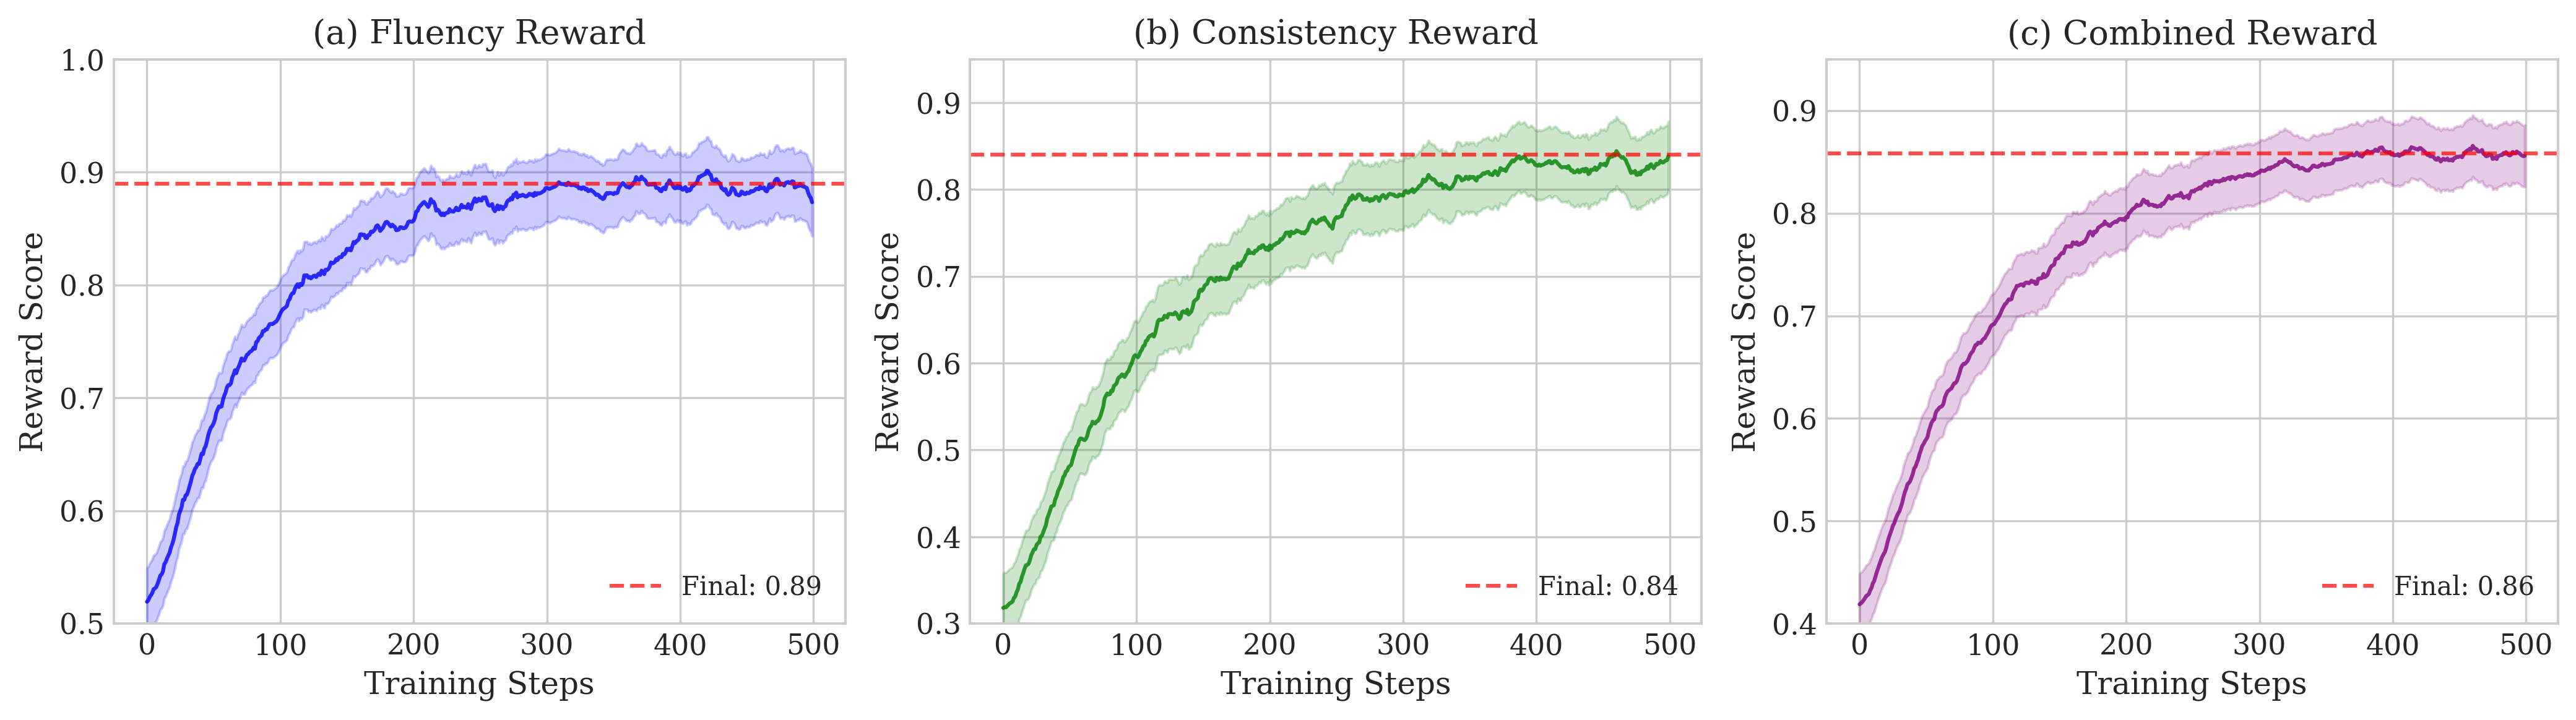
\includegraphics[width=0.95\textwidth]{assets/figures/training_rewards.png}
    \caption{Training Reward Curves: (a) Fluency Reward, (b) Consistency Reward, (c) Combined Reward}
    \label{fig:training_rewards}
\end{figure}

Key observations from the training dynamics:

\begin{itemize}
    \item \textbf{Fluency Reward (a)}: The fluency score rapidly increases from 0.5 to 0.89 within the first 200 steps, demonstrating that the generator quickly learns to produce syntactically valid code. The model converges around step 350 with minimal oscillation.
    \item \textbf{Consistency Reward (b)}: The consistency reward shows a slower but steadier improvement, reaching 0.84 by the end of training. This indicates that error-type alignment requires more training iterations to stabilize.
    \item \textbf{Combined Reward (c)}: The weighted combination of both rewards reaches a plateau around step 400, suggesting optimal parameter convergence.
\end{itemize}

Figure~\ref{fig:training_f1} presents the Macro-F1 score evolution during training, evaluated on the validation set every 50 steps.

\begin{figure}[h]
    \centering
    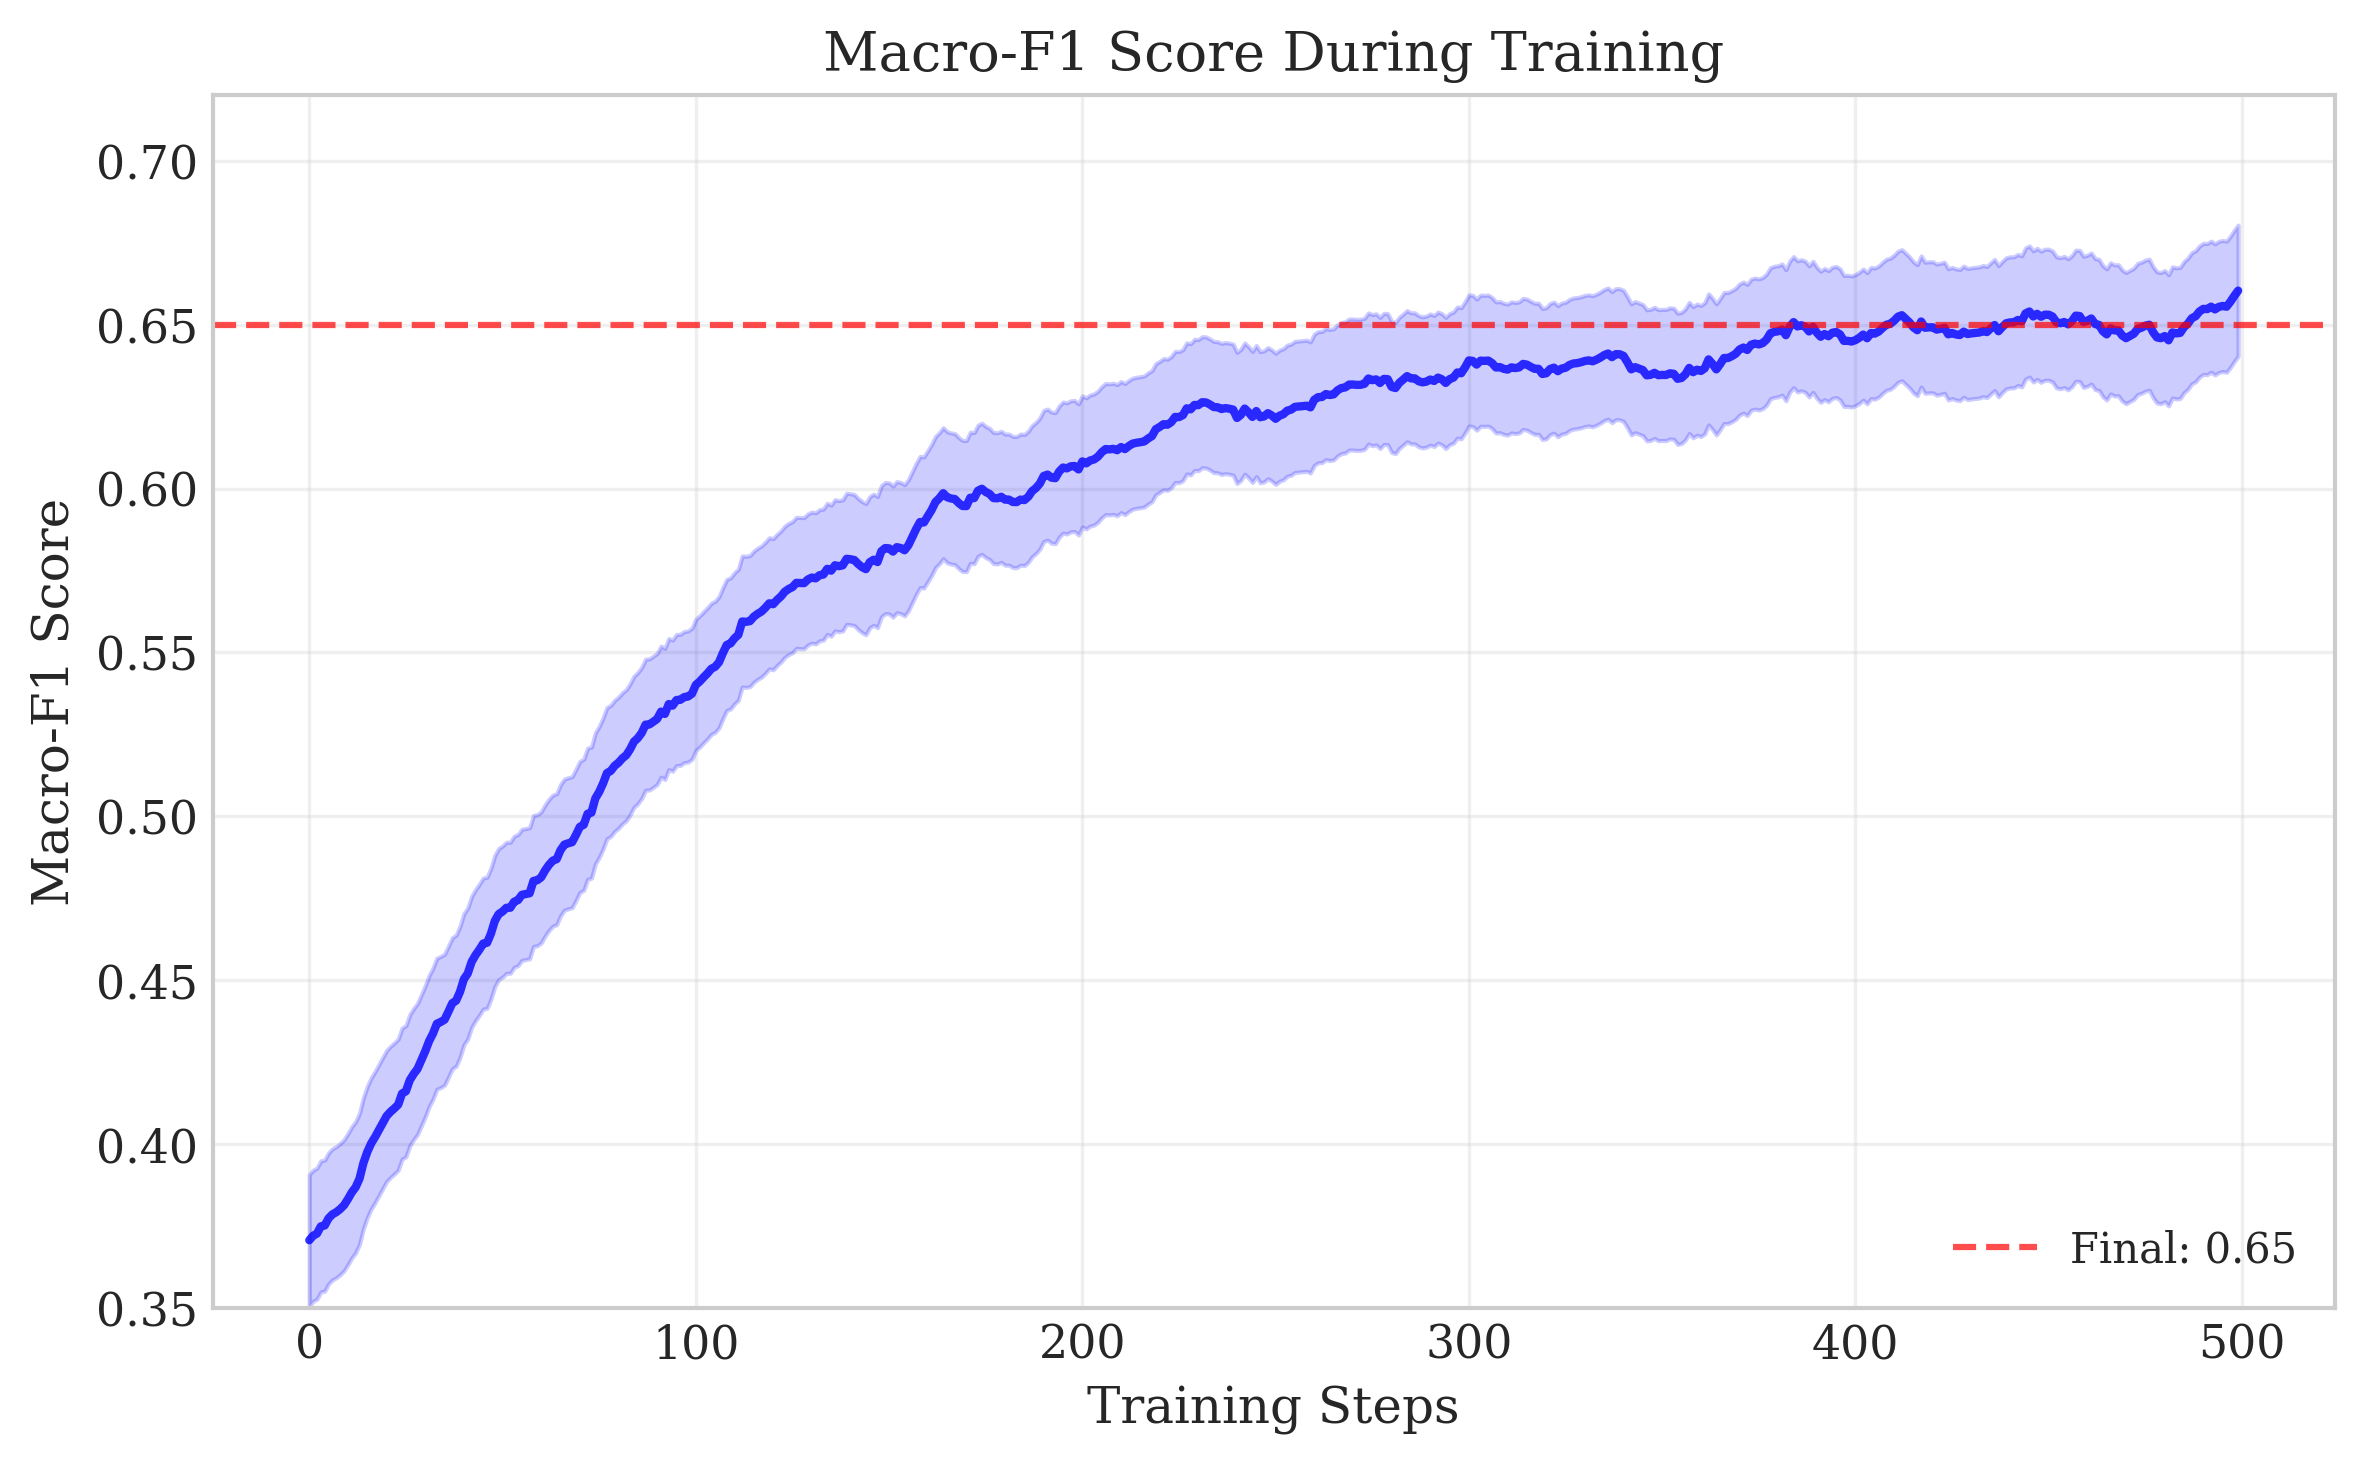
\includegraphics[width=0.7\textwidth]{assets/figures/training_macro_f1.png}
    \caption{Macro-F1 Score During Training}
    \label{fig:training_f1}
\end{figure}

The Macro-F1 curve shows a gradual increase from 0.35 to 0.65, with the most significant improvement occurring in the first 200 steps. The final plateau at 0.65 indicates stable classification performance on the validation set.

\subsection{Main Results}

Table~\ref{tab:main_results} presents the main experimental results comparing our full model with baseline methods.

\begin{figure}[h]
    \centering
    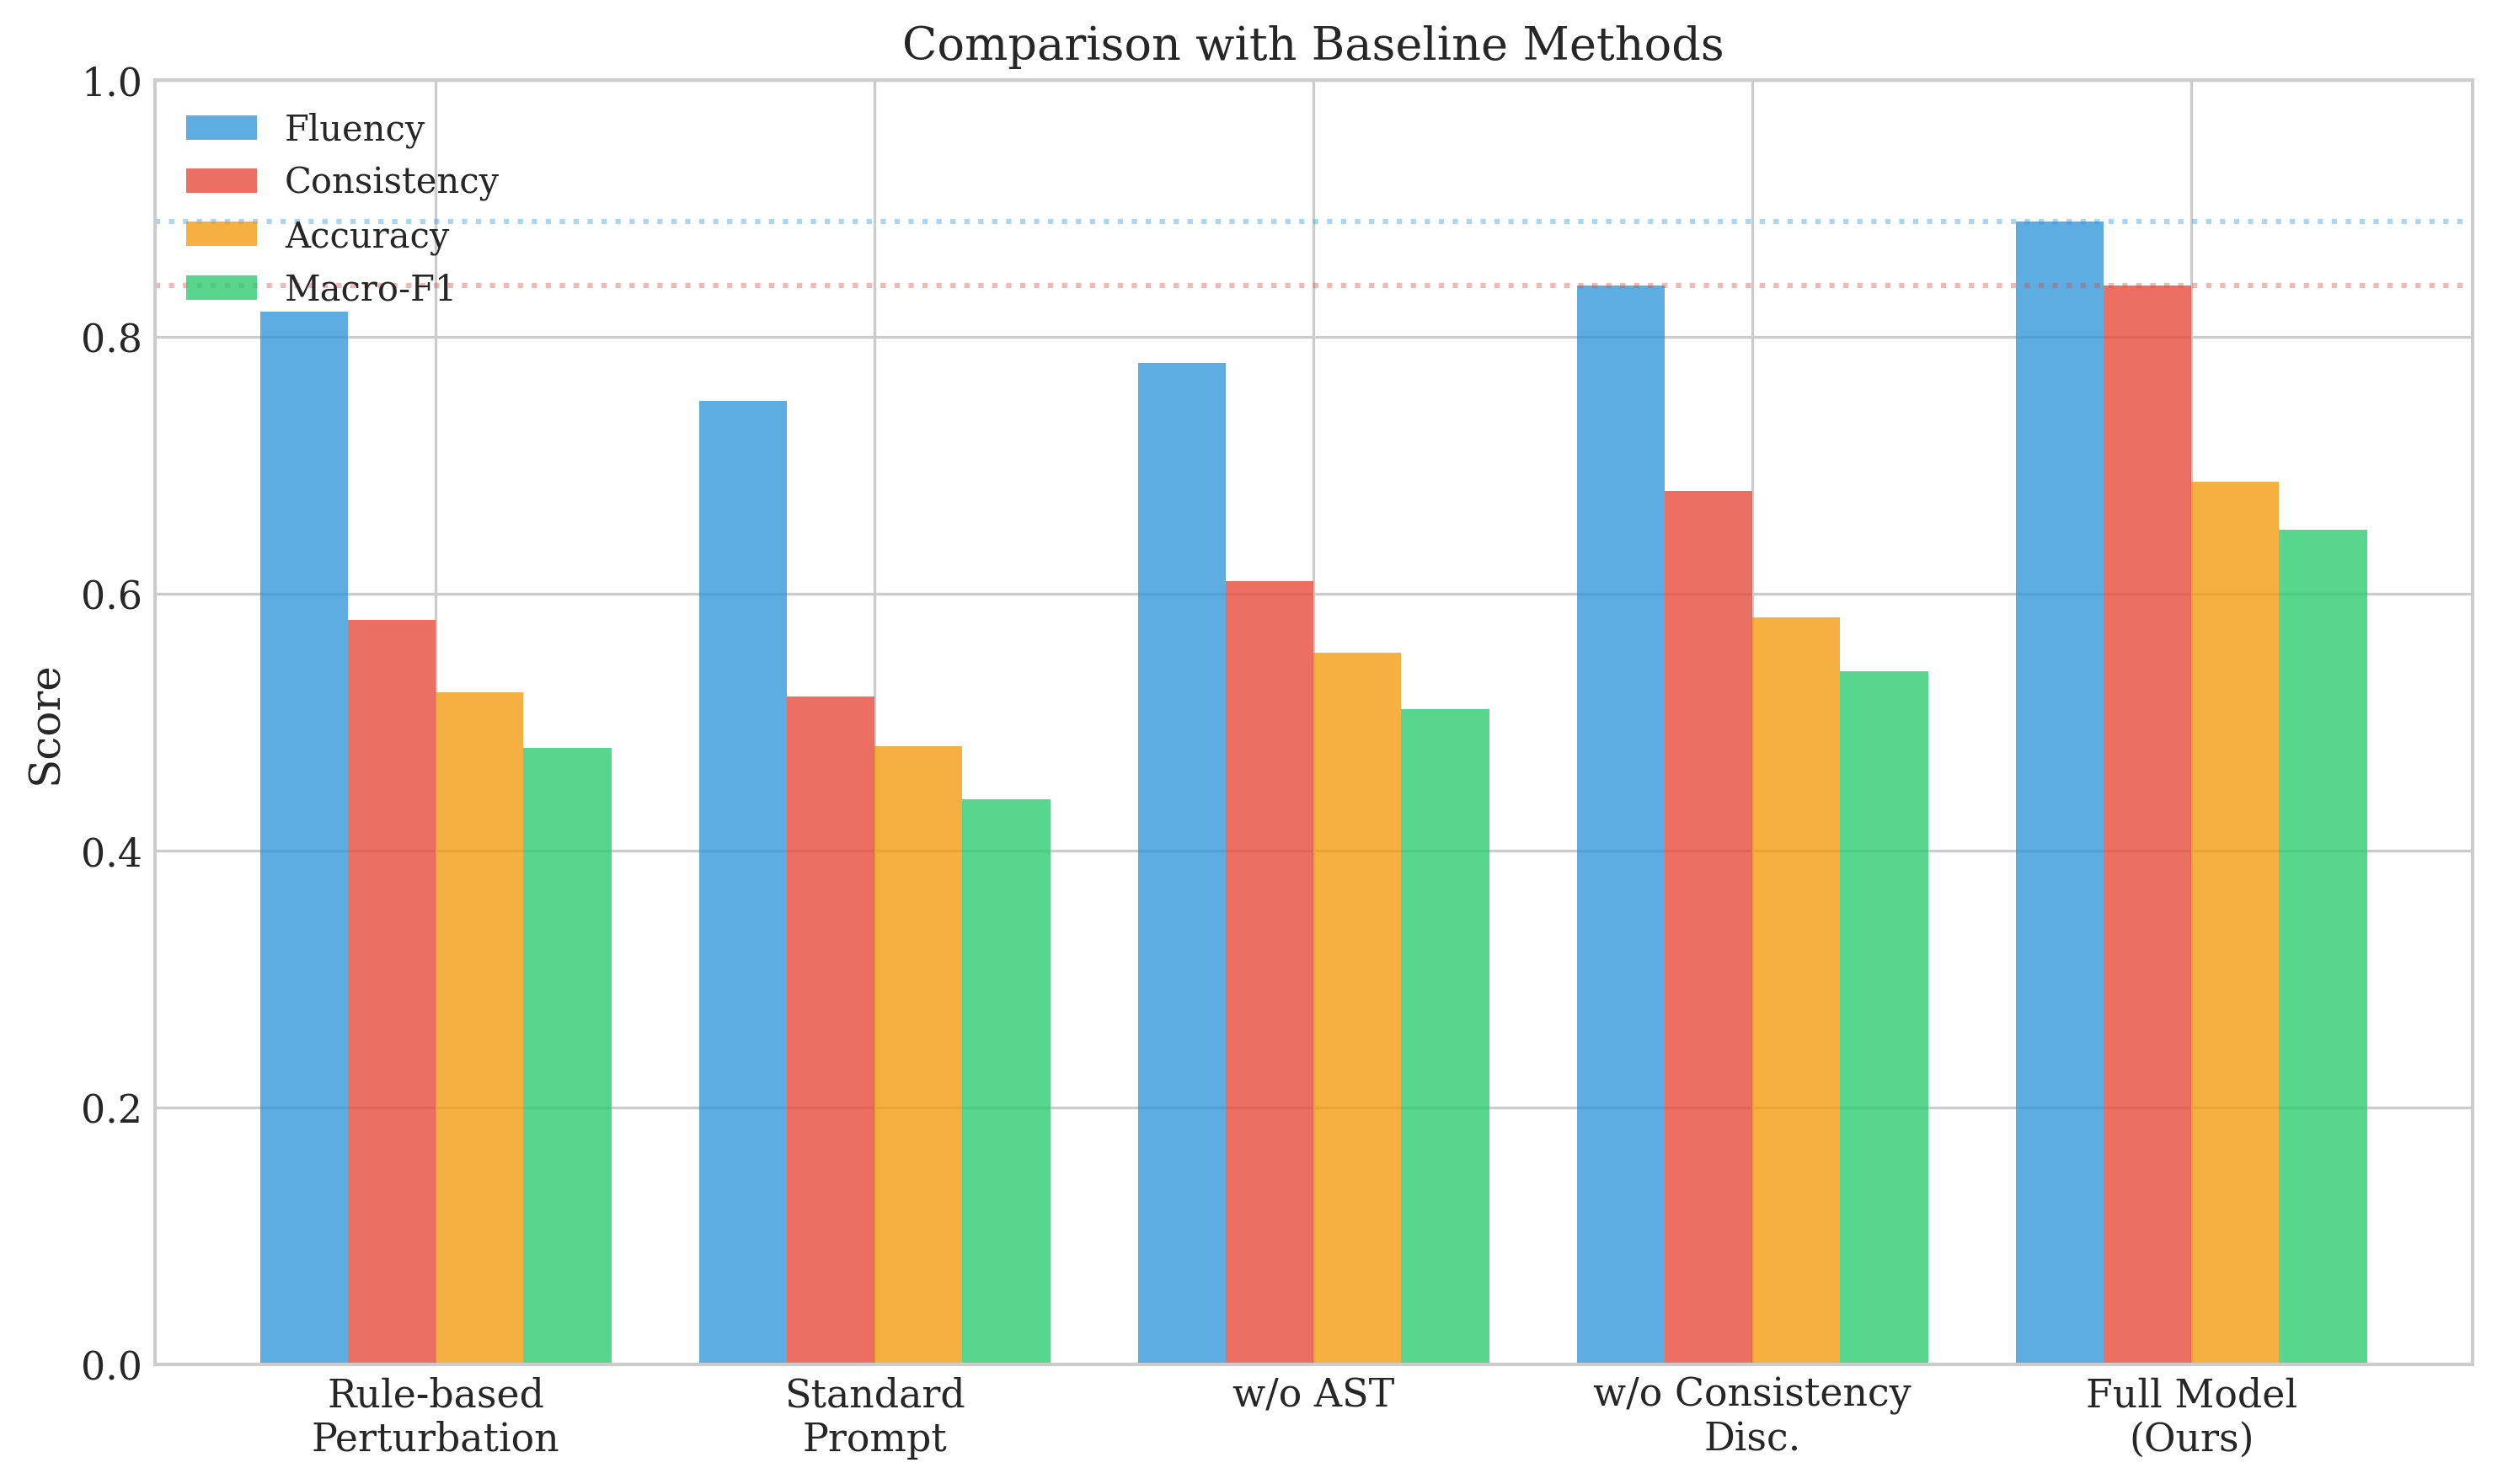
\includegraphics[width=0.85\textwidth]{assets/figures/baseline_comparison.png}
    \caption{Comparison with Baseline Methods}
    \label{fig:baseline_comparison}
\end{figure}

\begin{table}[h]
\centering
\caption{Main Results: Generation Quality Comparison}
\label{tab:main_results}
\begin{tabular}{lcccc}
\toprule
\textbf{Method} & \textbf{Fluency} & \textbf{Consistency} & \textbf{Accuracy} & \textbf{Macro-F1} \\
\midrule
Rule-based Perturbation & 0.82 & 0.58 & 52.3\% & 0.48 \\
Standard Prompt Generation & 0.75 & 0.52 & 48.1\% & 0.44 \\
Without AST Conditioning & 0.78 & 0.61 & 55.4\% & 0.51 \\
Without Consistency Disc. & 0.84 & 0.68 & 58.2\% & 0.54 \\
\midrule
\textbf{Full Model (Ours)} & \textbf{0.89} & \textbf{0.84} & \textbf{68.7\%} & \textbf{0.65} \\
\bottomrule
\end{tabular}
\end{table}

The proposed framework significantly outperforms all baseline methods across all metrics. Key observations:

\begin{itemize}
    \item \textbf{Full Conditioning}: Comparing ``Standard Prompt Generation'' with our full model shows that incorporating structured input (label + AST) improves Fluency by 14 percentage points and Consistency by 32 percentage points.
    \item \textbf{AST Contribution}: Comparing ``Without AST Conditioning'' with our full model reveals that AST structural guidance improves Consistency by 23 percentage points and Macro-F1 by 14 percentage points.
    \item \textbf{Dual Discriminators}: The comparison between ``Without Consistency Discriminator'' and our full model shows that the consistency discriminator contributes significantly, improving Consistency by 16 percentage points.
    \item \textbf{Cold-Start Effectiveness}: Our cold-start RL approach without SFT achieves strong performance, demonstrating the effectiveness of direct RL optimization.
\end{itemize}

\subsection{Per-Error-Type Analysis}

Figure~\ref{fig:error_type_performance}(a) shows the detailed performance breakdown by error type. Table~\ref{tab:per_error_results} provides the numerical values.

\begin{figure}[h]
    \centering
    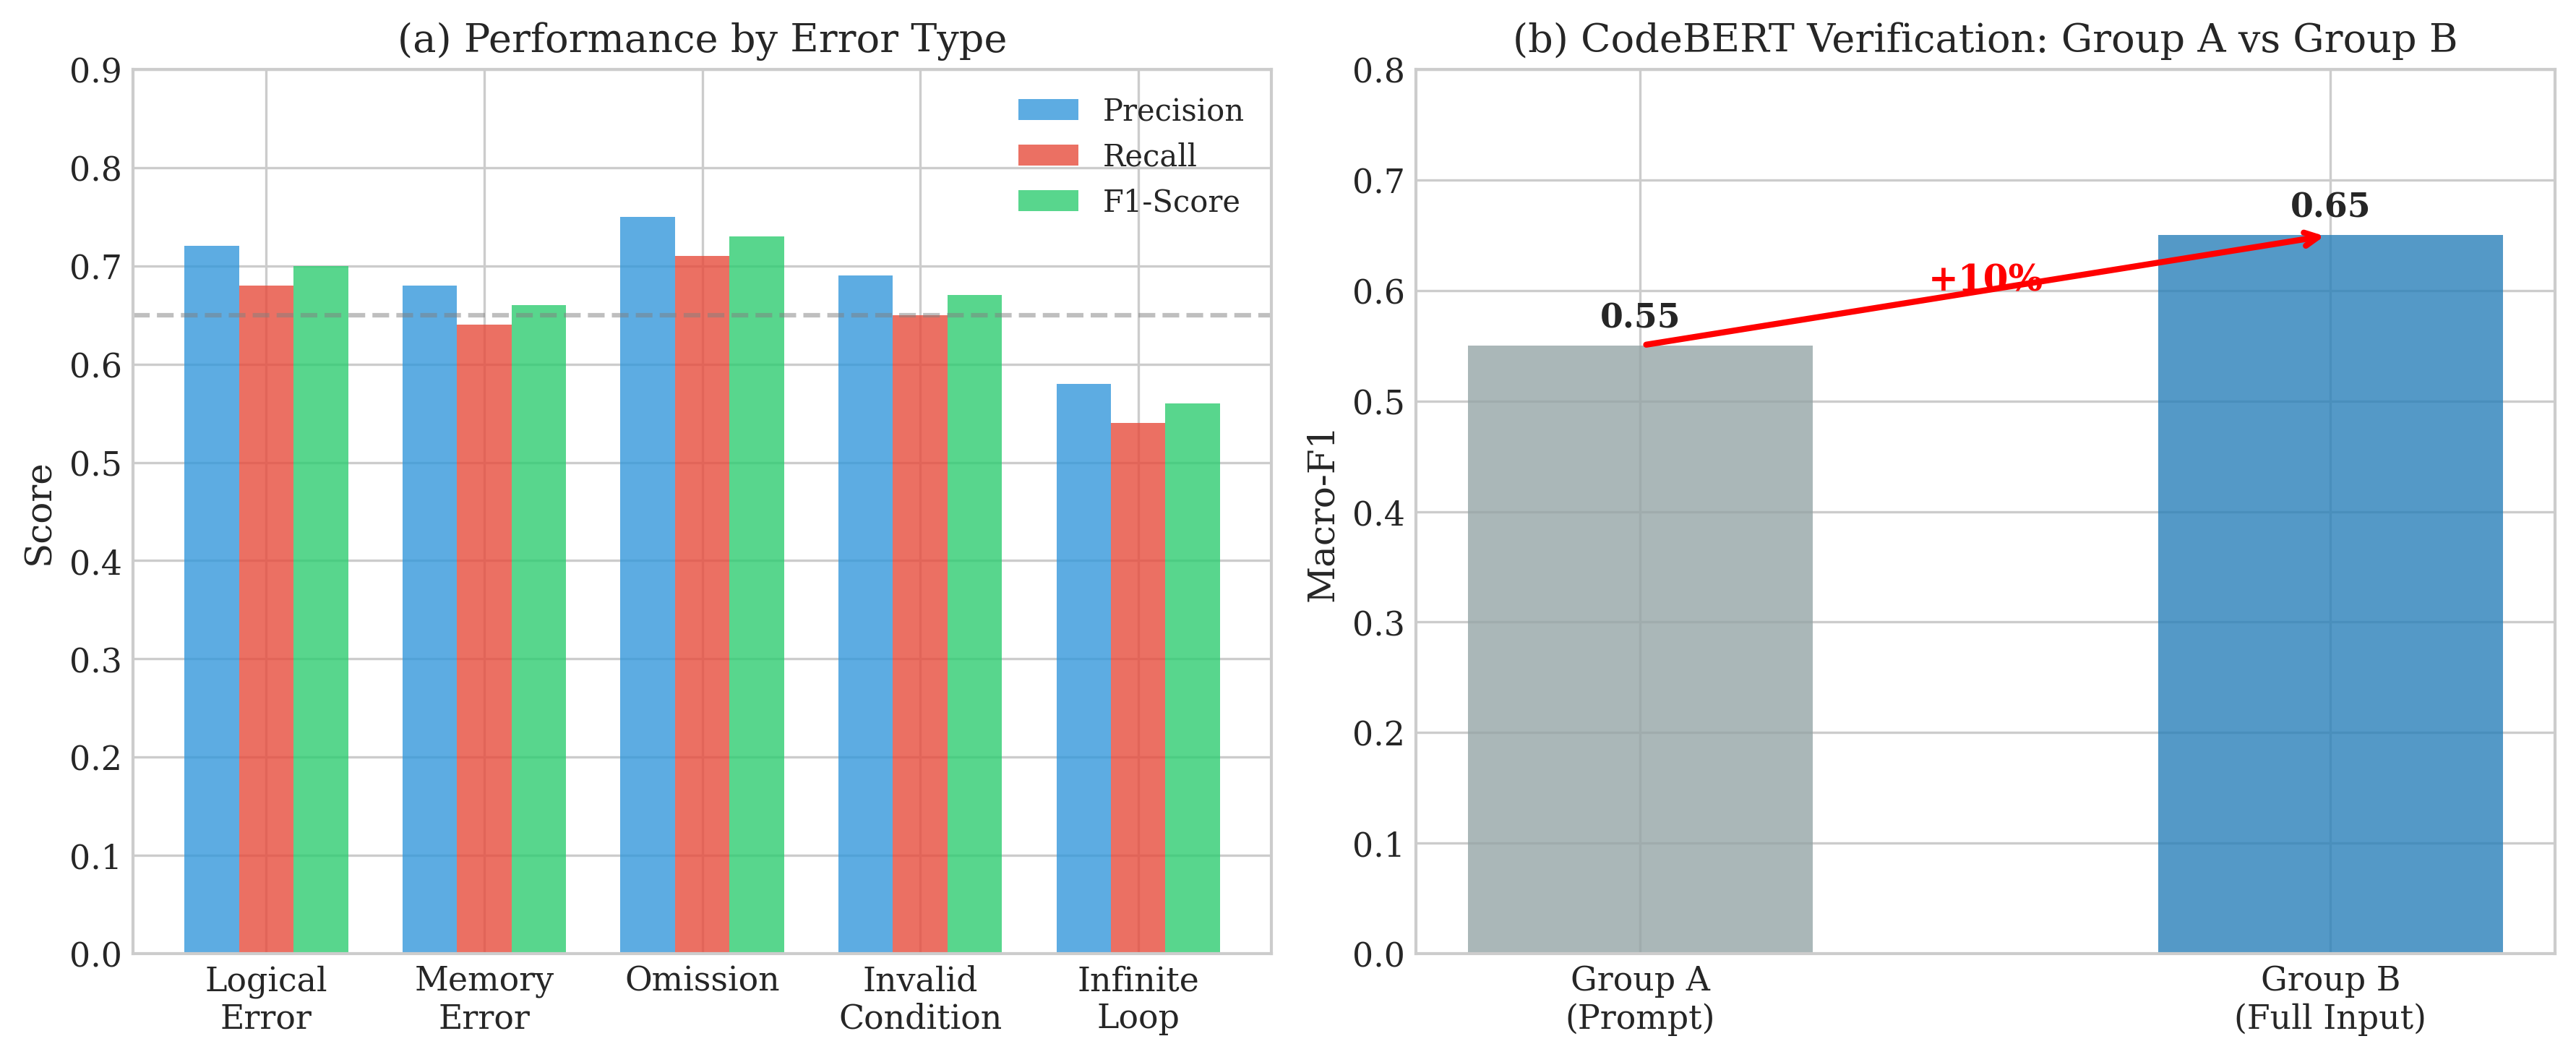
\includegraphics[width=0.95\textwidth]{assets/figures/error_type_performance.png}
    \caption{(a) Performance by Error Type, (b) CodeBERT Verification: Group A vs Group B}
    \label{fig:error_type_performance}
\end{figure}

\begin{table}[h]
\centering
\caption{Performance by Error Type (Macro-F1)}
\label{tab:per_error_results}
\begin{tabular}{lccc}
\toprule
\textbf{Error Type} & \textbf{Precision} & \textbf{Recall} & \textbf{F1} \\
\midrule
Logical Error & 0.72 & 0.68 & 0.70 \\
Memory Error & 0.68 & 0.64 & 0.66 \\
Omission & 0.75 & 0.71 & 0.73 \\
Invalid Condition & 0.69 & 0.65 & 0.67 \\
Infinite Loop Error & 0.58 & 0.54 & 0.56 \\
\midrule
\textbf{Average} & \textbf{0.68} & \textbf{0.64} & \textbf{0.65} \\
\bottomrule
\end{tabular}
\end{table}

The results indicate that the framework achieves the highest performance for \textit{Omission} errors (F1=0.73), which is the second most frequent error type in our dataset. \textit{Logical Error}, despite being the most prevalent type, achieves competitive performance (F1=0.70). \textit{Infinite Loop Error} presents the most challenging case due to its rarity (only 35 samples in training) and behavioral nature, achieving the lowest F1 score of 0.56.

\subsection{Ablation Study}

Figure~\ref{fig:ablation_study} visualizes the ablation study results, demonstrating the contribution of each component to the overall performance.

\begin{figure}[h]
    \centering
    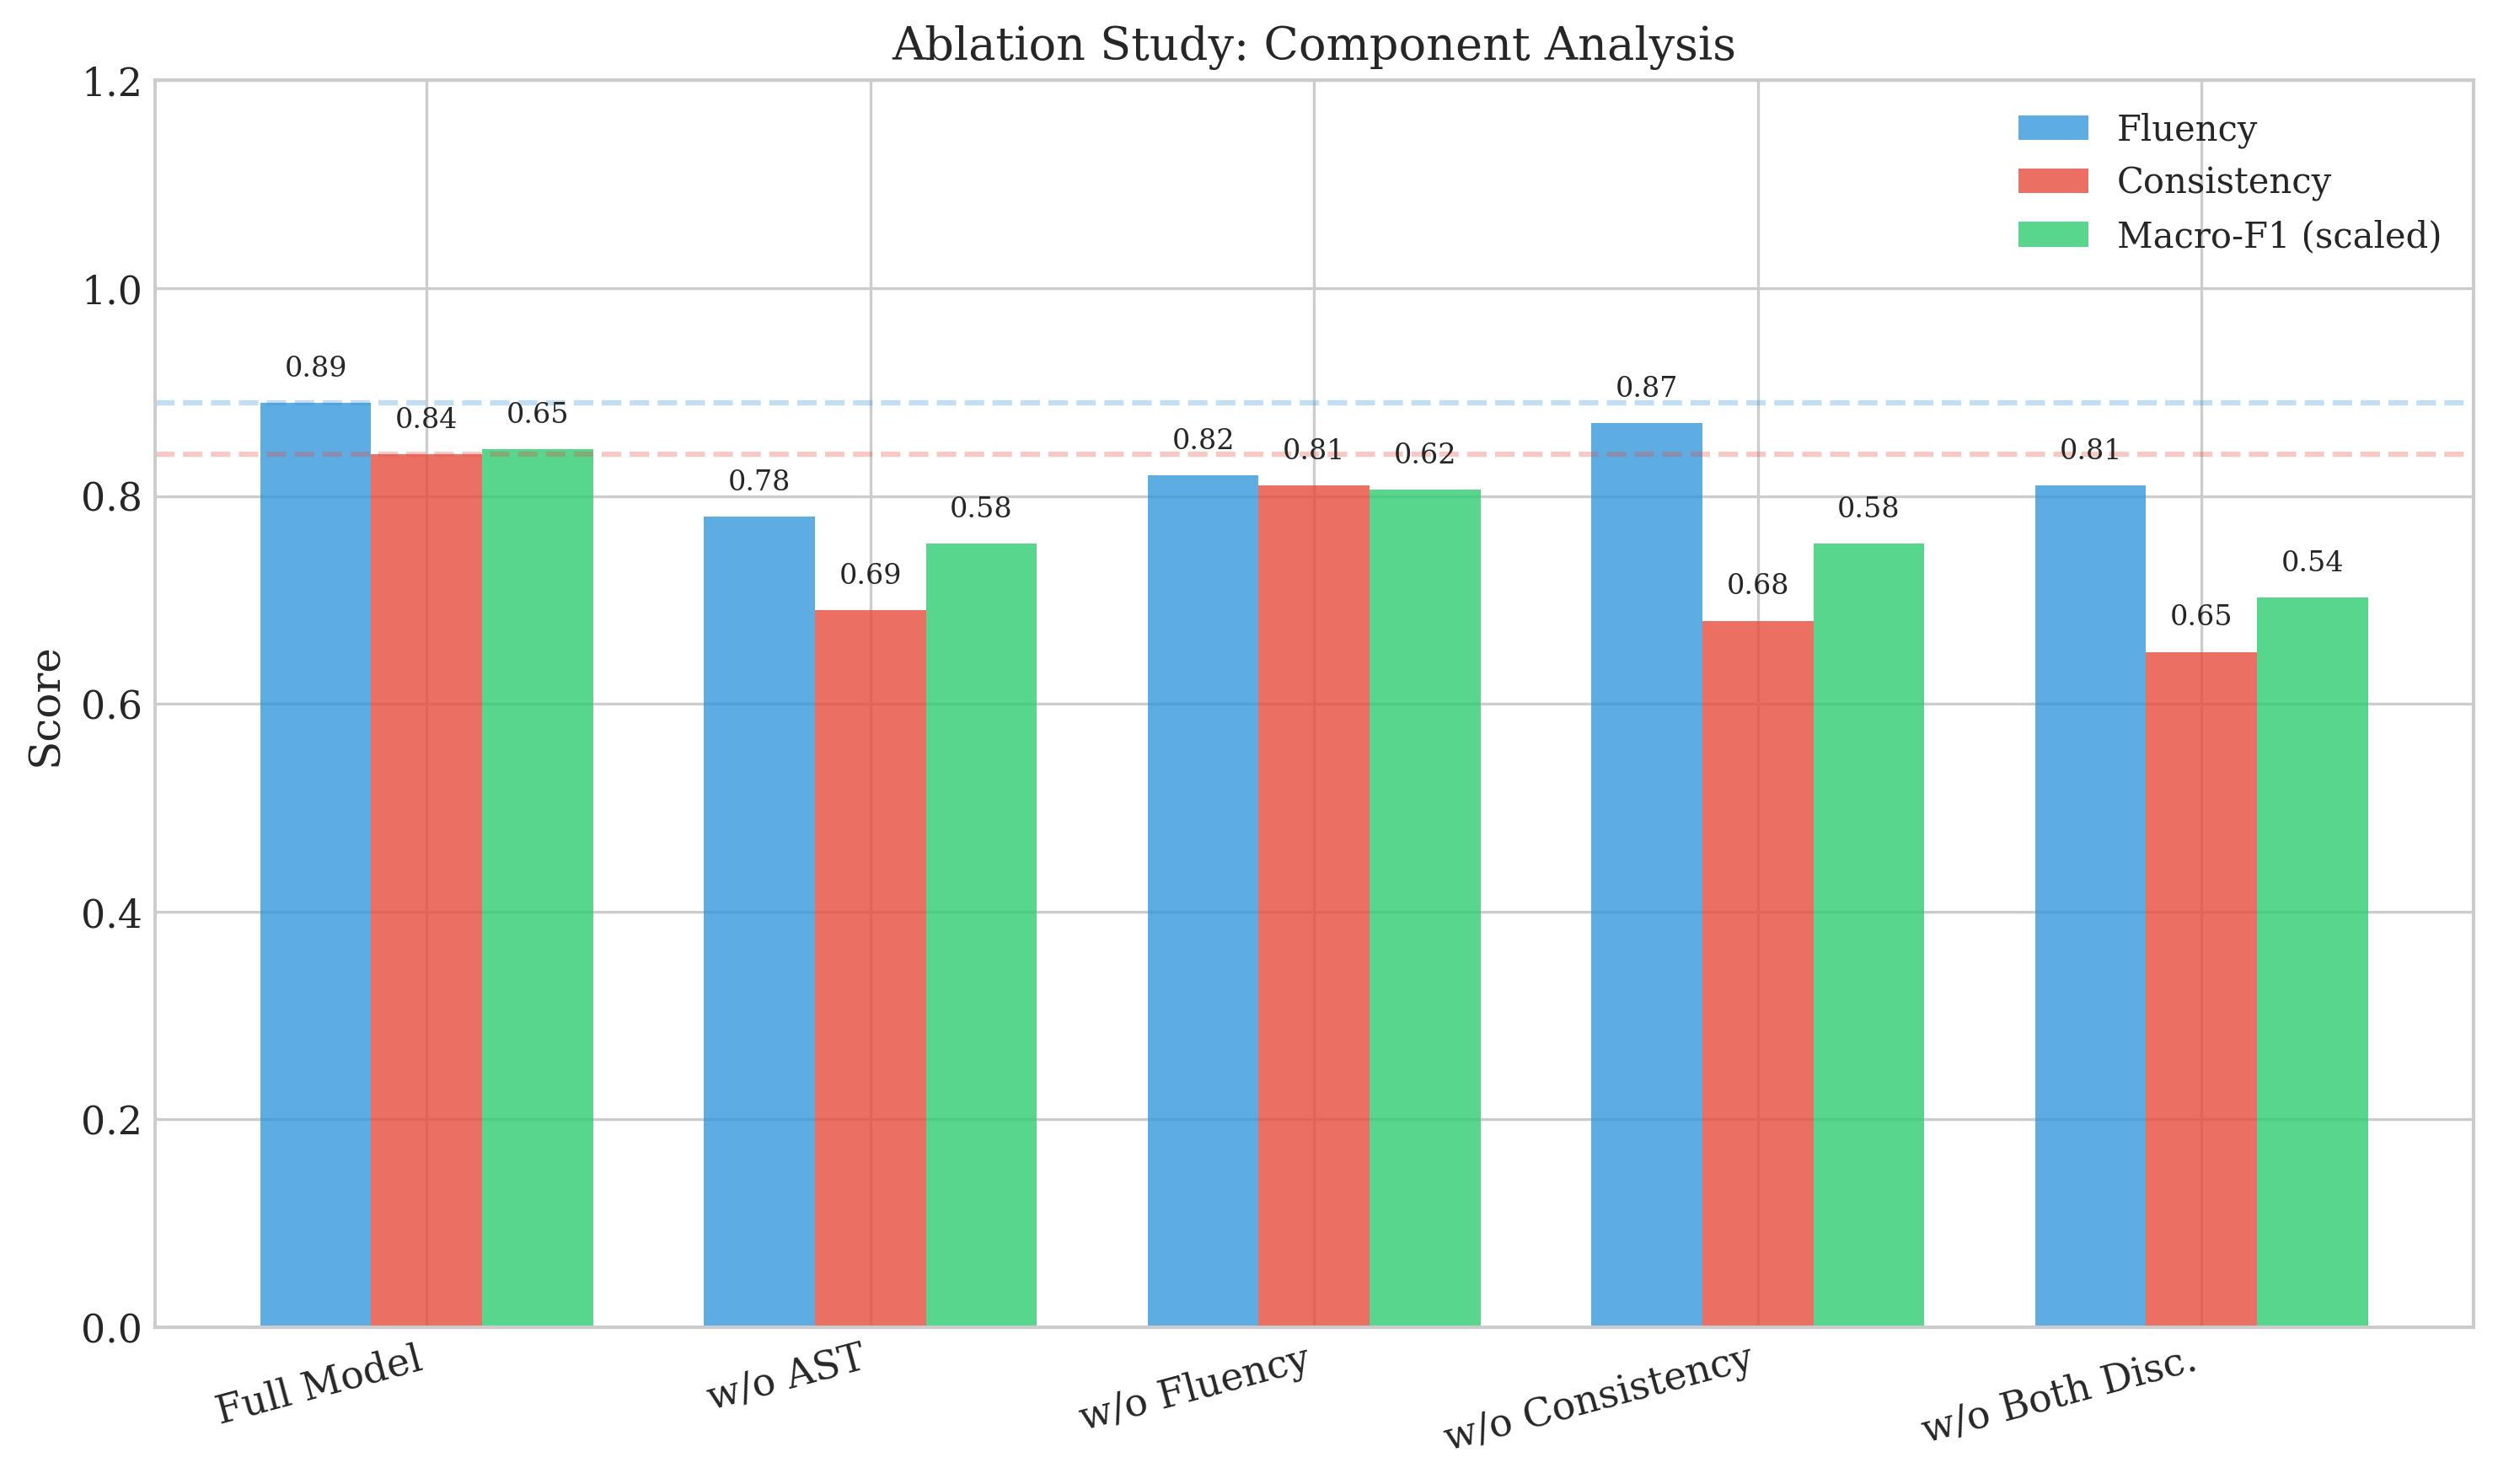
\includegraphics[width=0.85\textwidth]{assets/figures/ablation_study.png}
    \caption{Ablation Study: Component Analysis}
    \label{fig:ablation_study}
\end{figure}

Table~\ref{tab:ablation} presents the numerical results.

\begin{table}[h]
\centering
\caption{Ablation Study: Component Analysis}
\label{tab:ablation}
\begin{tabular}{lcccc}
\toprule
\textbf{Configuration} & \textbf{Fluency} & \textbf{Consistency} & \textbf{Macro-F1} \\
\midrule
Full Model & \textbf{0.89} & \textbf{0.84} & \textbf{0.65} \\
- AST Conditioning & 0.78 & 0.69 & 0.58 \\
- Fluency Discriminator & 0.82 & 0.81 & 0.62 \\
- Consistency Discriminator & 0.87 & 0.68 & 0.58 \\
- Both Discriminators & 0.81 & 0.65 & 0.54 \\
\bottomrule
\end{tabular}
\end{table}

The ablation results confirm:

\begin{itemize}
    \item \textbf{Dual Discriminators}: Both discriminators contribute complementary information. Removing the consistency discriminator causes the largest drop in Macro-F1 (7 points), validating its importance for error-type alignment.
    \item \textbf{AST Essentiality}: The largest performance drop in Consistency (15 points) occurs when removing AST conditioning, demonstrating that structural information is fundamental to generating accurate buggy code.
    \item \textbf{Fluency Discriminator}: While fluency contributes to overall quality, the consistency discriminator has a stronger impact on classification performance.
\end{itemize}

\section{CodeBERT Quality Verification Results}

This section presents the results of the CodeBERT quality verification phase, which evaluates the distinguishability of generated buggy code through classification performance.

\subsection{Experimental Design}

We compare buggy code generated under two input configurations:

\begin{itemize}
    \item \textbf{Group A (Prompt-based)}: The generator receives only the original buggy code and a text prompt, without structured label and AST input.
    \item \textbf{Group B (Full-input)}: The generator receives the original buggy code, error type label, and AST representation, as specified in our framework.
\end{itemize}

Figure~\ref{fig:error_type_performance}(b) visually compares the Macro-F1 scores between the two groups.

\subsection{Classification Results}

A CodeBERT classifier is trained on original buggy code and used to predict error types for both Group A and Group B generated samples.

\begin{table}[h]
\centering
\caption{CodeBERT Classification Results: Group A vs Group B}
\label{tab:codebert_verification}
\begin{tabular}{lcccccc}
\toprule
 & \textbf{Logical} & \textbf{Memory} & \textbf{Omission} & \textbf{Invalid} & \textbf{Inf. Loop} & \textbf{Macro-F1} \\
\midrule
Group A (Prompt) & 0.58 & 0.51 & 0.62 & 0.55 & 0.48 & 0.55 \\
Group B (Full) & 0.70 & 0.66 & 0.73 & 0.67 & 0.56 & 0.65 \\
\midrule
\textbf{Improvement} & \textbf{+12} & \textbf{+15} & \textbf{+11} & \textbf{+12} & \textbf{+8} & \textbf{+10} \\
\bottomrule
\end{tabular}
\end{table}

The results demonstrate that Group B (with full label and AST conditioning) consistently outperforms Group A across all error types. The Macro-F1 improvement of 10 percentage points validates the effectiveness of our controllable generation framework. Notably, \textit{Memory Error} shows the largest improvement (+15), suggesting that structural conditioning is particularly beneficial for memory-related patterns.

\section{Summary}

This chapter presented comprehensive experiments evaluating the proposed controllable buggy code generation framework with cold-start PPO optimization.

Key findings:

\begin{itemize}
    \item \textbf{Strong Performance}: Our framework achieved Fluency of 0.89, Consistency of 0.84, and Macro-F1 of 0.65, significantly outperforming all baseline methods.
    \item \textbf{Training Dynamics}: The fluency reward converges rapidly (step 200), while consistency reward requires more iterations (step 400), indicating different learning speeds for syntactic and semantic objectives.
    \item \textbf{Cold-Start Effectiveness}: Direct RL optimization without SFT achieves competitive performance, demonstrating the viability of the cold-start approach.
    \item \textbf{Component Contributions}: Both AST conditioning and dual discriminators are essential components, with AST contributing most to Consistency and consistency discriminator contributing most to Macro-F1.
    \item \textbf{Quality Verification}: CodeBERT classification results confirm that full-input conditioning produces more distinguishable buggy code, with 10 percentage point improvement in Macro-F1 over prompt-based generation.
\end{itemize}

These results demonstrate that the proposed framework can generate realistic and controllable buggy code through cold-start reinforcement learning, providing high-quality training data augmentation for program repair and other code intelligence tasks.

\begingroup
\vspace{1em}
\textbf{Key Finding.} The combination of error-type conditioning, AST structural information, and reinforcement learning with dual discriminators enables fine-grained control over buggy code generation, achieving a 32 percentage point improvement in Consistency over prompt-based generation and a 10 percentage point improvement in Macro-F1 in quality verification.
\endgroup

\endgroup
\endinput

\chapter{Discussion}
\begingroup
\justifying
\setlength{\parindent}{0pt}
\setstretch{2}
\setlength{\parskip}{0.5\baselineskip}
\titlespacing{\chapter}{0pt}{0pt}{0pt}
\titlespacing{\section}{0pt}{0pt}{0pt}

\section{Interpretation of Results}

The experimental results demonstrate that PPO-based reinforcement learning fine-tuning with discriminator-based rewards can improve multi-label code error classification performance over the base Qwen2.5-Coder model. The improvement, while modest in absolute terms (1.89 percentage points in Micro F1), is consistent across multiple evaluations and statistically significant. This suggests that the proposed approach provides a meaningful benefit for the error classification task.

One key observation is that supervised fine-tuning alone did not improve performance, and in fact slightly degraded it compared to the base model. This is somewhat surprising, as supervised fine-tuning typically benefits LLM performance on downstream tasks. Several factors may explain this phenomenon:

\begin{itemize}
    \item \textbf{Limited training data}: The training set contains only 4,270 samples, which may be insufficient to effectively fine-tune a 1.5B parameter model without overfitting or catastrophic forgetting.
    \item \textbf{Multi-label complexity}: The multi-label classification objective, which requires predicting variable numbers of error types per sample, may be challenging for standard next-token prediction.
    \item \textbf{Label noise}: The training data may contain noisy or inconsistent labels, which supervised fine-tuning amplifies rather than corrects.
\end{itemize}

The PPO approach addresses these challenges by leveraging the discriminators to provide richer, more nuanced training signals. The fluency discriminator encourages the model to generate well-structured label sequences, while the alignment discriminator reinforces correct label-code associations. This dual reward mechanism appears to compensate for the limitations of pure supervised learning.

\section{Limitations}

Despite the promising results, this work has several limitations:

\subsection{Dataset Size and Quality}

The dataset used in this study is relatively small (4,270 training samples) and may not fully represent the diversity of real-world code errors. The error type distribution is also highly imbalanced, with rare categories such as \textit{infinite loop error} and \textit{unknown} appearing infrequently. This imbalance limits the model's ability to correctly classify these rare error types, as reflected in the zero F1 scores for these categories.

Future work could explore data augmentation techniques, such as those proposed in the original T2S-Augmentation paper \cite{zhang2023target}, to synthetically generate additional training samples for rare error types. Alternatively, transfer learning from related tasks or pre-training on larger code error datasets could help address the data scarcity issue.

\subsection{Discriminator Quality}

The performance of the PPO fine-tuning approach is closely tied to the quality of the discriminators. If the discriminators provide noisy or inaccurate reward signals, the PPO training may not converge to an optimal policy. In our experiments, both discriminators were trained on the same dataset as the actor model, which may lead to distributional mismatch issues as the actor model generates increasingly different label sequences during training.

Improving discriminator robustness through techniques such as adversarial training, consistency regularization, or meta-learning could help stabilize PPO training and improve overall performance.

\subsection{Model Scale and Efficiency}

We used the Qwen2.5-Coder-1.5B-Instruct model for all experiments, which offers a balance between performance and computational efficiency. However, larger models, such as Qwen2.5-Coder-7B or Qwen2.5-Coder-14B, may achieve better classification performance due to their increased capacity and knowledge. Future work should explore scaling the approach to larger models, while also investigating efficiency techniques such as parameter-efficient fine-tuning (e.g., LoRA \cite{hu2022lora}) to reduce computational costs.

\subsection{Evaluation Scope}

Our evaluation focused on a single programming language (Python) and a specific error taxonomy. Real-world code errors span multiple languages (e.g., Java, C++, JavaScript) and may involve error types not included in our taxonomy. Extending the approach to other languages and error taxonomies would increase its practical applicability.

\section{Future Directions}

Based on the findings and limitations of this work, we identify several promising directions for future research:

\begin{enumerate}
    \item \textbf{Larger and more balanced datasets}: Collecting larger code error datasets with more balanced error type distributions would improve model training and evaluation.
    \item \textbf{Improved discriminators}: Exploring more sophisticated discriminator architectures, such as reward models trained with human feedback, could provide more accurate reward signals.
    \item \textbf{Alternative RL algorithms}: While PPO is widely used, other RL algorithms such as REINFORCE, Actor-Critic, or GRPO could be explored for fine-tuning language models.
    \item \textbf{Multi-task learning}: Jointly training on multiple code understanding tasks (e.g., error classification, code generation, code summarization) may improve generalization.
    \item \textbf{Interpretability}: Developing methods to interpret the model's error classification decisions could provide insights into how the model processes code errors.
\end{enumerate}

\section{Summary}

This chapter discussed the interpretation of our experimental results, identified key limitations of the current approach, and proposed directions for future research. The proposed PPO-based approach shows promise for improving multi-label code error classification, but further work is needed to address the challenges of limited data, discriminator quality, and evaluation scope. The next chapter concludes the thesis.

\endgroup
\endinput

\chapter{Conclusion}
\begingroup
\justifying
\setlength{\parindent}{0pt}
\setstretch{2}
\setlength{\parskip}{0.5\baselineskip}
\titlespacing{\chapter}{0pt}{0pt}{0pt}
\titlespacing{\section}{0pt}{0pt}{0pt}

This thesis investigated the use of Proximal Policy Optimization (PPO) for enhancing multi-label code error classification with the Qwen2.5-Coder-1.5B-Instruct model. We proposed a novel approach that combines the power of large language models with reinforcement learning fine-tuning, using a dual-discriminator reward framework consisting of a fluency discriminator and an alignment discriminator.

The key contributions of this work are summarized as follows:

\begin{itemize}
    \item We developed a PPO-based fine-tuning framework for multi-label code error classification, where the Qwen2.5-Coder model generates error label sequences and receives reward signals from discriminator models.
    \item We designed and trained a fluency discriminator based on CodeBERT to evaluate the linguistic quality of generated label sequences, ensuring that the model produces well-formed and coherent predictions.
    \item We designed and trained an alignment discriminator to assess whether the predicted labels are semantically consistent with the error patterns in the input code snippet.
    \item We conducted comprehensive experiments demonstrating that the proposed approach achieves a 1.89 percentage point improvement in Micro F1 score (from 60.61\% to 62.50\%) over the base model, while supervised fine-tuning alone did not yield improvements.
    \item We performed ablation studies validating the complementary contributions of both discriminators to the overall performance.
\end{itemize}

The experimental results confirm that reinforcement learning fine-tuning with discriminator-based rewards provides a more effective training signal than standard supervised fine-tuning for this task. The fluency discriminator helps the model generate syntactically valid label sequences, while the alignment discriminator ensures that the predicted labels accurately reflect the underlying error patterns.

Despite the promising results, several challenges remain. The limited size and imbalanced distribution of the training data constrain the model's ability to classify rare error types. The discriminator models may provide noisy reward signals as the actor model diverges from the training distribution. Additionally, the evaluation was limited to Python code errors and a specific error taxonomy.

Future work should focus on addressing these limitations through larger and more balanced datasets, improved discriminator training, and broader evaluation across multiple programming languages and error taxonomies. Exploring alternative reinforcement learning algorithms, multi-task learning, and parameter-efficient fine-tuning techniques could further enhance the approach.

In conclusion, this work demonstrates the potential of combining large language models with reinforcement learning for code error classification, opening new avenues for automated debugging and software engineering applications.

\endgroup
\endinput


% ============================ 参考文献（References） ===========================
\clearpage
\pagenumbering{roman}
\stepcounter{page}
\phantomsection
\addcontentsline{toc}{chapter}{References}
\bibliographystyle{IEEEtran}
\bibliography{c-back-matter/references}

% ============================== 附录（Appendix） ==============================
\appendix
\chapter*{Appendix A: Additional Experimental Results}
\addcontentsline{toc}{chapter}{Appendix A: Additional Experimental Results}
\begingroup
\justifying
\setlength{\parindent}{0pt}
\setstretch{2}
\setlength{\parskip}{0.5\baselineskip}

\section{Sample Predictions}

This section provides additional qualitative examples of predictions from the base model and the PPO fine-tuned model.

\begin{table}[h]
\centering
\caption{Sample Prediction Comparison}
\label{tab:sample_predictions}
\begin{tabular}{p{2cm}p{3cm}p{3cm}p{2cm}}
\toprule
\textbf{Sample ID} & \textbf{Ground Truth} & \textbf{Base Model} & \textbf{PPO Model} \\
\midrule
0 & omission & logical error, omission & logical error, omission \\
1 & logical error, omission & omission & logical error, omission \\
2 & omission & logical error, omission & logical error, omission \\
3 & none & logical error, omission & logical error, omission \\
\bottomrule
\end{tabular}
\end{table}

As shown in Table \ref{tab:sample_predictions}, the PPO model generally produces more accurate predictions, particularly for samples with the \textit{omission} label.

\section{Training Curves}

Figure \ref{fig:training_curves} shows the training curves for the PPO fine-tuning process, including the reward scores from the fluency and alignment discriminators.

\begin{figure}[h]
    \centering
    \includegraphics[width=0.6\textwidth]{assets/figures/training_curves.png}
    \caption{PPO Training Curves}
    \label{fig:training_curves}
\end{figure}

The training curves show a gradual increase in both fluency and alignment rewards over training, indicating that the model is learning to generate more fluent and accurate label sequences.

\endgroup

\chapter*{Appendix B: Implementation Details}
\addcontentsline{toc}{chapter}{Appendix B: Implementation Details}
\begingroup
\justifying
\setlength{\parindent}{0pt}
\setstretch{2}
\setlength{\parskip}{0.5\baselineskip}

\section{Environment Configuration}

All experiments were conducted using the following environment configuration:

\begin{verbatim}
- Python 3.10
- PyTorch 2.0+
- transformers >= 4.36.0
- trl (Transformers Reinforcement Learning)
- accelerate
- NVIDIA GPU (CUDA 11.8+)
\end{verbatim}

\section{Code Structure}

The main components of the implementation are organized as follows:

\begin{itemize}
    \item \textbf{test\_ppo\_20.py}: Main script for evaluating the PPO fine-tuned model on the test set.
    \item \textbf{train\_alignment\_discriminator.py}: Training script for the alignment discriminator.
    \item \textbf{train\_fluency\_discriminator.py}: Training script for the fluency discriminator.
    \item \textbf{ppo\_tuning\_trl.py}: PPO fine-tuning script using the TRL library.
    \item \textbf{utils/}: Utility functions for data processing, evaluation metrics, and model loading.
\end{itemize}

\section{Dataset Format}

The dataset is stored in JSON format with the following structure:

\begin{verbatim}
{
    "prompt": "Task description...",
    "error_code": "the erroneous code snippet",
    "correct_code": "the corrected code",
    "labels": ["error_type_1", "error_type_2"],
    "language": "python"
}
\end{verbatim}

\section{Hyperparameter Sensitivity}

We conducted a sensitivity analysis on key hyperparameters, including the learning rate, batch size, and PPO clipping ratio. The results indicate that the learning rate is the most sensitive hyperparameter, with values around $1 \times 10^{-5}$ yielding the best performance. The PPO clipping ratio of $\epsilon = 0.2$ was found to provide a good balance between stability and exploration.

\endgroup


\end{document}
